\documentclass[a4paper,12pt]{memoir}

% Includes
\usepackage{epsfig}
\usepackage{graphicx}
\usepackage{amsmath}
\usepackage{amssymb}
\usepackage{algorithm}
\usepackage{algpseudocode}
\usepackage{rotating}
\usepackage{caption}
\usepackage{subcaption}
\usepackage{enumitem}
\usepackage{multirow}
\usepackage{epigraph}
\usepackage{pgfplots}
\usepackage{upgreek}
\usepackage{adjustbox}
\usepackage{gensymb}
\usepackage{xfrac}
\usepackage{pdflscape}
\usepackage{afterpage}
\usepackage{tabularx}
\newcolumntype{Y}{>{\centering\arraybackslash}X}
\usepackage[noabbrev,capitalize]{cleveref}
\newcommand{\norm}[1]{\left\lVert #1 \right\rVert}
% Custom macros
\newcommand{\fig}[1]{Figure~\ref{fig:#1}}
\newcommand{\tbl}[1]{Table~\ref{tbl:#1}}
\newcommand{\sct}[1]{Section~\ref{sec:#1}}
\newcommand{\eqn}[1]{(\ref{eqn:#1})}
\newcommand{\todo}[1]{\textcolor{red}{TODO: #1}\PackageWarning{TODO:}{#1!}}

\usepackage{pifont}% http://ctan.org/pkg/pifont
\newcommand{\cmark}{\ding{51}}%
\newcommand{\xmark}{\ding{55}}%
% Math
\newcommand{\N}{\mathcal{N}}
\newcommand{\f}{\mathbf{f}}
\newcommand{\x}{\mathbf{x}}
\newcommand{\Bb}{\mathbf{b}}
\newcommand{\y}{\mathbf{y}}
\newcommand{\z}{\mathbf{z}}
\newcommand{\W}{\mathbf{W}}
\newcommand{\X}{\mathbf{X}}
\newcommand{\Y}{\mathbf{Y}}
\newcommand{\softmax}{\text{Softmax}}
\newcommand{\cL}{\mathcal{L}}
\newcommand{\Wh}{{\widehat{\mathbf{W}}}}
\newcommand{\diag}{\text{diag}}
\newcommand{\p}{\mathbf{p}}

% ********************************** Preamble **********************************
% Preamble: Contains packages and user-defined commands and settings
% **************************** Custom Packages ********************************
\let\newfloat\undefined
\usepackage{algorithm}
\usepackage{algpseudocode}
\usepackage{amsfonts}       % blackboard math symbols
\usepackage{amsmath}
\usepackage{amssymb}
\usepackage{bbm}  % for \mathbbm{1}
\usepackage{bibentry}
\nobibliography*
\usepackage{bm}  % for more powerful bold symbols https://tex.stackexchange.com/a/596
\usepackage{booktabs}
\usepackage{breakcites}
\usepackage{pifont}  % for dingbats checkmark and xmark
\usepackage{mathtools}
\usepackage{ifthen}
\usepackage{keyval}
\usepackage{placeins}
\usepackage{tabu}
\usepackage{tikz}
\usepackage[normalem]{ulem}
\usepackage{upgreek}

% If you comment hyperref and then uncomment it, you should delete
% egpaper.aux before re-running latex.  (Or just hit 'q' on the first latex
% run, let it finish, and you should be clear).
\usepackage[pagebackref=true,breaklinks=true,letterpaper=true,colorlinks,bookmarks=false]{hyperref}

\usetikzlibrary{arrows.meta, backgrounds, calc, fit, positioning}

\DeclareMathOperator*{\binop}{\oplus}


% *************************** Graphics and figures *****************************

% Uncomment the following two lines to force Latex to place the figure.
% Use [H] when including graphics. Note 'H' instead of 'h'
%\usepackage{float}
%\restylefloat{figure}

% \usepackage{subcaption}

% ********************************** Tables ************************************
\usepackage{booktabs} % For professional looking tables
% \usepackage{multirow}

%\usepackage{multicol}
%\usepackage{longtable}
%\usepackage{tabularx}


% *********************************** SI Units *********************************
\usepackage{siunitx} % use this package module for SI units


% ******************************* Line Spacing *********************************

% Choose linespacing as appropriate. Default is one-half line spacing as per the
% University guidelines

% \DoubleSpacing
\setuogspacing{\OnehalfSpacing}
% \SingleSpacing


% ************************ Formatting / Footnote *******************************

% Don't break enumeration (etc.) across pages in an ugly manner (default 10000)
%\clubpenalty=500
%\widowpenalty=500

%\usepackage[perpage]{footmisc} %Range of footnote options


% *****************************************************************************
% *************************** Bibliography  and References ********************

%\usepackage{cleveref} %Referencing without need to explicitly state fig /table

% Add `custombib' in the document class option to use this section

% changes the default name `Bibliography` -> `References'
\renewcommand{\bibname}{References}


% ******************************** Roman Pages *********************************
% The romanpages environment set the page numbering to lowercase roman one
% for the contents and figures lists. It also resets
% page-numbering for the remainder of the dissertation (arabic, starting at 1).

\newenvironment{romanpages}{
  \setcounter{page}{1}
  \renewcommand{\thepage}{\roman{page}}}
{\newpage\renewcommand{\thepage}{\arabic{page}}}


% ******************************************************************************
% ************************* User Defined Commands ******************************
% ******************************************************************************

\makeatletter                  % You do not need to write [htpb] all the time
\renewcommand\fps@figure{htbp} %
\renewcommand\fps@table{htbp}  %
\makeatother                   %

% *********** To change the name of Table of Contents / LOF and LOT ************

%\renewcommand{\contentsname}{My Table of Contents}
%\renewcommand{\listfigurename}{My List of Figures}
%\renewcommand{\listtablename}{My List of Tables}
\DeclarePairedDelimiter\ceil{\lceil}{\rceil}
\DeclarePairedDelimiter\floor{\lfloor}{\rfloor}
\newcommand{\matr}[1]{#1}
\newcommand{\tens}[1]{\mathcal{#1}}
\renewcommand{\vec}[1]{#1}
\newcommand{\vect}[2]{\vec{#1}^{(#2)}}

% Generalized hadamard product fusion
\newcommand{\thetavec}{\ensuremath{\theta}}
\newcommand{\fusop}{\ensuremath{\mathcal{F_{\thetavec}}}}
\newcommand{\mutanfeat}[1]{\ensuremath{\tilde{#1}}}
\newcommand{\m}{\ensuremath{m}}
\newcommand{\n}{\ensuremath{n}}
\newcommand{\q}{\ensuremath{q}}
\renewcommand{\v}{\ensuremath{v}}
\newcommand{\z}{\ensuremath{z}}
\newcommand{\A}{\ensuremath{A}}
\newcommand{\B}{\ensuremath{B}}
\renewcommand{\C}{\ensuremath{C}}
\newcommand{\R}{\ensuremath{\mathbb{R}}}
\newcommand{\T}{\ensuremath{\mathcal{T}}}
\newcommand{\Tfibre}{\ensuremath{\T_{i_1 \cdots i_{n - 1} \,:\, i_{n + 1} \cdots i_N}}}
\newcommand{\TsizeIn}[1]{\ensuremath{I_1 \times \cdots \times I_{n - 1} \times #1 \times I_{n + 1} \times \cdots \times I_N}}
\newcommand{\binopb}{\ensuremath{\sideset{}{_b}\binop}}
\newcommand{\binopseq}{\ensuremath{{(\binopb)}_{b = 1}^B}}
\newcommand{\binoppartition}{\ensuremath{{\{\tuckbranch\}}_b}}
\newcommand{\binoppartB}{\ensuremath{\mathbb{B}}}
\newcommand{\binoppartBseq}{\ensuremath{{(\binoppartB_b)}_{b = 1}^B}}
\newcommand{\tuckbranch}{\ensuremath{\T_r^{\q{}\v{}}}}
\newcommand{\hadamardqv}{\ensuremath{N_r\mutanfeat{q} \odot M_r\mutanfeat{v}}}

% SST
\newcommand{\real}{\mathbb{R}}
\newcommand{\yvosvalG}{68.1}
\newcommand{\davisvalG}{53.2}
\newcommand{\inputvar}{\mathcal{X}}
\newcommand{\outputvar}{\mathcal{Y}}
\newcommand{\vidfeat}{\mathcal{T}}
\newcommand{\objfeat}{\mathcal{R}}
\newcommand{\pixel}{p}
\newcommand{\querytensor}{\mathcal{Q}}
\newcommand{\keytensor}{\mathcal{K}}
\newcommand{\embtensor}{\mathcal{E}}
\newcommand{\valuetensor}{\mathcal{V}}
\newcommand{\objmean}{\mu_o}
\newcommand{\objcov}{\Sigma_o}
\newcommand{\objctx}{\tilde{\mu}_o}
\newcommand{\viddim}{\real{}^{C\times T\times H\times W}}
\newcommand{\softmax}{\mathtt{softmax}}
\newcommand{\yesmark}{\ding{51}}
\newcommand{\nomark}{\ding{55}}
\newcommand{\J}{$\mathcal{J}$}
\newcommand{\F}{$\mathcal{F}$}
\renewcommand{\G}{$\mathcal{G}$}
\newcommand{\JandF}{$\mathcal{J} \& \mathcal{F}$}


% ********************************* Appendix ***********************************

% The default value of both \appendixtocname and \appendixpagename is `Appendices'. These names can all be changed via:

%\renewcommand{\appendixtocname}{List of appendices}
%\renewcommand{\appendixname}{Appndx}


% ************************ Thesis Information & Meta-data **********************
% Thesis title and author information, refernce file for biblatex
% ************************ Thesis Information & Meta-data **********************
%% The title of the thesis
\title{Learning Fusion Operators for Multiple Modality Machine Learning}
%\texorpdfstring is used for PDF metadata. Usage:
%\texorpdfstring{LaTeX_Version}{PDF Version (non-latex)} eg.,
%\texorpdfstring{$sigma$}{sigma}

%% Subtitle (Optional)
% \subtitle{}

%% The full name of the author
\author{Brendan Duke}

%% Department (eg. Department of Engineering, Maths, Physics)
% \dept{Department of Engineering}

%% University and Crest
% \university{University of Guelph}
% Crest minimum should be 30mm.
% \crest{
\includegraphics[width=0.2\textwidth]{UofGshield}}
%% Use this crest, if you are using the college crest
%% Crest long miminum should be 65mm
%\crest{\includegraphics[width=0.45\textwidth]{University_Crest_Long}}

%% College shield [optional] 
% Crest minimum should be 30mm.
%\collegeshield{\includegraphics[width=0.2\textwidth]{CollegeShields/Kings}}


%% Supervisor (optional)
%\supervisor{Prof. Kenichi Soga}
%% Supervisor Role (optional) - Supervisor (default) or advisor
%\supervisorrole{Advisor: }

%% Advisor (optional)
%\advisor{Prof. Malcolm Bolton}
%% Advisor Role (optional) - Advisor (default) or leave empty
%\advisorrole{Advisor: }


%% You can redefine the submission text:
% Default as per the University guidelines:
% ``This dissertation is submitted for the degree of''
%\renewcommand{\submissiontext}{change the default text here if needed}

%% Full title of the Degree
% \degreetitle{Master of Applied Science}

%% College affiliation (optional)
% \college{Trinity College}

%% Submission date
% Default is set as {\monthname[\the\month]\space\the\year}
% \degreedate{August 2019}

%% Meta information
% \subject{Computer Vision} \keywords{{Deep Learning} {Visual Question Answering} {Fusion} {Multi-modal} {Activity Recognition} {Neural Architecture Search}}


% ******************************** Front Matter ********************************
\begin{document}

\frontmatter

\begin{titlepage}
  \maketitle
\end{titlepage}

% % ******************************* Thesis Dedidcation ********************************

\begin{dedication}

% ``It is not the mountain we conquer but ourselves.''
% 
% \textit{Sir Edmund Hillary (1919 - 2008)}

\end{dedication}

% ******************************* Thesis Declaration ***************************

\begin{declaration}

I hereby declare that except where specific reference is made to the work of 
others, the contents of this dissertation are original and have not been 
submitted in whole or in part for consideration for any other degree or 
qualification in this, or any other university. This dissertation is my own 
work and contains nothing which is the outcome of work done in collaboration 
with others, except as specified in the text and Acknowledgements. This 
dissertation contains fewer than 65,000 words including appendices, 
bibliography, footnotes, tables and equations and has fewer than 150 figures.

% Author and date will be inserted automatically from thesis.tex \author \degreedate

\end{declaration}

% % ************************** Thesis Acknowledgements **************************
I would like to thank my advisor, Dr. Graham Taylor, and the rest of the MLRG
lab for their mentorship and providing an environment where I could learn how
to do research.
I came to the University of Guelph without a research background.
Dr. Taylor and the MLRG members were patient and allowed me to gradually find
my own process for doing research, while providing helpful advice and
discussions that continue through today.
I am thankful that I had the opportunity to work with this group of bright,
kind, motivated people and I hope our collaborations will continue into the
future.

I would also like to thank our academic collaborators from the Deep Vision
project, who are fantastic role models for how to be good scientists.
In particular I would like to thank Dr. Christian Wolf, who provided thoughtful
insight and ideas about our work as well as the machine learning and computer
vision fields in general.

Finally, I would like to thank Shannon Despond for her constant loving support
throughout my studies.

% ************************** Thesis Abstract *****************************
% Use `abstract' as an option in the document class to print only the titlepage and the abstract.
In this thesis by articles we make contributions related to attention and
fusion in the intersection of the deep learning and computer vision fields.

In our first article, we investigated the design of neural network operators
that fuse features extracted from different modalities, such as audio and
video, and use the fused representation to make predictions on a single task,
such as visual question answer or activity recognition.
We propose a generalized class of multimodal fusion operators for the task of
visual question answering (VQA).
We identify generalizations of existing multimodal fusion operators based on
the Hadamard product, and show that specific non-trivial instantiations of this
generalized fusion operator exhibit superior performance in terms of OpenEnded
accuracy on the VQA task.
In particular, we introduce Nonlinearity Ensembling, Feature Gating, and
post-fusion neural network layers as fusion operator components, culminating in
an absolute percentage point improvement of~$1.1\%$ on the VQA~2.0 test-dev set
over baseline fusion operators, which use the same features as input.
We use our findings as evidence that our generalized class of fusion operators
could lead to the discovery of even superior task-specific operators when used
as a search space in an architecture search over fusion operators.

In our second article, we introduced Transformers, which are an attention-based
architecture, to the video object segmentation (VOS) task.
Video Object Segmentation (VOS) requires tracking an object through a video
with pixel-level accuracy, and has previously been solved either through
combinations of online fine-tuning or recurrent feature propagation, which have
inherent disadvantages.
Online fine-tuning methods have slow runtime, while recurrent methods lack
scalability and have the drawback of compounding error, due to their sequential
nature.
We propose a scalable, end-to-end method for VOS called
``Sparse Spatiotemporal Transformers'' (SST) to address said runtime,
scalability and temporal dependency issues.
SST extracts per-pixel representations for each object by simultaneously
attending to high semantic information feature vectors at each pixel in a
video.
SST performs inference in a single feedforward pass of a Transformer
architecture designed with sparse attention components.
We contribute the first method for using attention-based networks for VOS, and
demonstrate the scalability advantage of attention-based over recurrent
networks in the spatiotemporal domain.
We show that our attention-based feedforward method achieves competitive
results on YouTube-VOS 2019 and DAVIS2017 at a fraction of the runtime of state
of the art approaches.
% TODO(brendan): runtime + scalability numbers from on-device profiling.


% *********************** Adding TOC and List of Figures ***********************

\tableofcontents

\listoffigures

\listoftables

% \printnomenclature[space] space can be set as 2em between symbol and description
%\printnomenclature[3em]

\printnomenclature

% ******************************** Main Matter *********************************
\mainmatter

\chapter{BACKGROUND}

Our work concerns the investigation of complex computer vision problems, and in
one article the relation of vision and natural language, using the method of
extracting deep hierarchical representations known as deep learning.
Underpinning the methods in our articles are a set of deep learning
architectures, each of which constitutes its own active topic of research.
After briefly describing deep learning as a whole, we introduce the particular
subcomponents underlying our models, in order to provide additional background
context before presenting our articles.


\section{Deep Learning}

Deep learning is a subfield of machine learning that uses a hierarchy of neural
network layers for representation learning~\cite{lecun2015deeplearning}.
Representation learning, then, means to extract from raw data meaningful
information in the form of vectors or tensors of real-valued numbers, called
``features''.
The defining quality of deep learning is its learning of a deep hierarchy of
representations using backpropagation~\cite{rumelhart1988learningreps}, which
is the term used by the deep learning community for reverse-mode automatic
differentation~\cite{griewank2008evaluatingderivatives}.
Thanks to breakthroughs in computation, data and algorithms, in recent years
deep learning methods have made progress in domains that had previously proven
challenging for traditional machine learning approaches.
Today, deep learning is a top-performing approach for solving complex
machine-learning problems including image and speech recognition, language
translation and natural language understanding topics such as question
answering~\cite{lecun2015deeplearning}.

We introduce feedforward neural networks (FNNs) as a simple yet concrete
example of a deep learning model.
FNNs can be expressed as a sequence of hidden layers
\begin{equation}
\vec{h}_i = f_i({\matr{W}_i}^\intercal \vec{h}_{i - 1} + \vec{b}_i),
\label{eqn:background:fnn}
\end{equation}
where $\vec{h}_i$ is a hidden unit, $\matr{W}_i$ is the weight matrix of
layer~$i$ of the neural network, $\vec{b}_i$ is a bias vector and $f_i$ is a
non-linearity or link function, such as the sigmoid
function~$f(x) = 1/(1 + e^{-x})$ or ReLU~$f(x) = \max(x, 0)$.
We may consider~$h_0$ as the input feature vector to the FNN, and~$h_L$ as the
output prediction for an FNN with~$L$ layers.
As with other deep models, the representation capacity of FNNs can be tuned by
increasing the depth of the network, i.e., the total number of layers of the
form in Equation~\ref{eqn:background:fnn}, or by increasing the width of each
of the layers~$i$, i.e., the dimension of the hidden
representation~$\vec{h}_i$.

In our articles we make use of more complex neural network architectures than
FNNs, which may include FNNs as a subcomponent.
In particular we focus on convolutional neural networks, recurrent neural
networks, attention networks, and fusion operators, all of which we describe
below.


\section{Convolutional Neural Networks}

Convolutional neural networks (CNNs) are a type of neural network designed to
model data that is arranged in a grid, as the pixels in an image are arranged.
While each neuron in a layer of an FNN is connected to all neurons in its
previous layer via a matrix multiplication, neurons in a layer of a CNN are
only locally connected to neurons in the previous layer.

We explain the meaning of ``locally connected''. We assume that a given layer
has a 3D tensor $\tens{V}$ as input, where in addition to the single dimension
of the hidden unit vector $\vec{h}$ of FNNs, there are two extra spatial
dimensions (e.g. $x$ and $y$ dimensions of an image).  A CNN connects the input
tensor $\tens{V}$ to an output tensor $\tens{Z}$ through a 4D tensor
$\tens{K}$ called a ``kernel'', which contains the CNN's learned parameters.

The kernel has one dimension matching the ``channels'' (the third, i.e.\
non-spatial, dimension of the input tensor $\tens{V}$), one dimension that
becomes the channels of the output tensor $\tens{Z}$, and two spatial
dimensions that are normally much smaller than the input feature tensor
$\tens{Z}$'s spatial dimensions. E.g.\ for an input image of dimensions $224
\times 224$ pixels and~\num{3} colour channels, a CNN kernel's spatial
dimensions would normally be $3 \times 3$. The CNN kernel's weights are thus
shared spatially, and each element of the output tensor is contributed to only
by a $3 \times 3$ spatial region of the input tensor, via a sum over
channel-wise matrix multiplications of the kernel strictly over that spatial
region.

Formally, each element $\tens{Z}_{i, j, k}$ of the output tensor corresponds to the
sum given in Equation~\ref{eqn:convolution}, where~$i$ is the index of the
output channel and $j$ and $k$ are the spatial indices of the output element.
The index~$l$ runs over the input channels, while~$m$ and $n$ are restricted by
the spatial dimensions of the kernel, e.g.\ in our $3 \times 3$ kernel example
we have $m, n \in \{-1, 0, 1\}$.

\begin{equation}
        \tens{Z}_{i, j, k} = \sum_{l, m, n} \tens{V}_{l, j + m, k + n} \tens{K}_{i, l, m, n}
\label{eqn:convolution}
\end{equation}

\begin{figure}
\centering
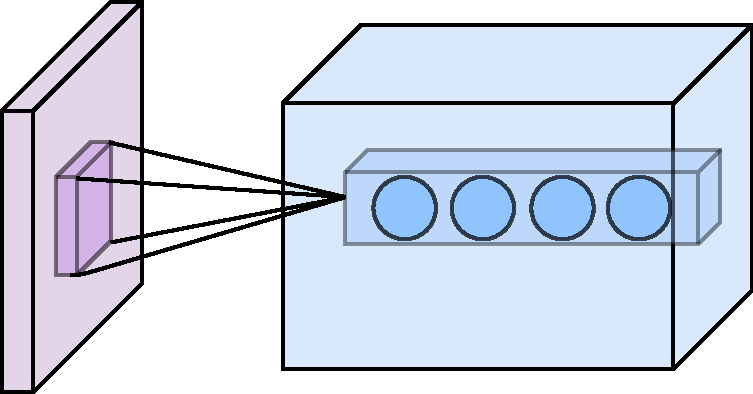
\includegraphics[width=1.0\textwidth]{Figures/cnn.pdf}
\caption{Two subsequent layers of a convolutional neural network.}
\label{fig:cnn}
\end{figure}

Figure~\ref{fig:cnn} depicts the interaction between two subsequent layers of a
CNN\@. The kernel~$\tens{K}$ (inner box on the left) is multiplied with a
volume of the input~$\tens{V}$ (outer box on the left) to produce a single unit
consisting of a column of values at a single spatial location in the
output~$\tens{Z}$.

CNNs generalize well in comparison to FNNs on visual data, since the number of
parameters are dramatically reduced compared with an equivalent FNN by sharing
parameters in the spatial dimensions~\cite{lecun-89}. This is an example of
improving generalization of neural networks by using prior knowledge (i.e.\ in
this case, the spatial equivariance of image data) when constructing a model
for a given type of data.

In the case of the visual question-answering task, we make use of a particular
CNN architecture called a ResNet~\cite{he2016deep} that has~\num{152} layers.
This CNN architecture has been pre-trained on a large dataset of image data to
extract useful generic feature representations from images.
The fusion operator takes this image feature representation as input, along
with a feature representation of the question, in order to predict an answer to
the posed question conditioned on the image.


\section{Recurrent Neural Networks}

Like CNNs, Recurrent Neural Networks~(RNNs)~\cite{rumelhart1986learning} are a
type of neural network model that has been designed using prior knowledge of
the type of data distribution relevant to the given task.
In particular, RNNs are designed to work on sequential data of arbitrary
length, such as time-series data including stock prices over time, or language
data, where the inputs are the word or character tokens making up sentences and
paragraphs.

Instead of sharing parameters spatially as in CNNs, RNNs share parameters over
time. The output at each timestep~$t$, $\vect{a}{t}$, takes as input both the
``hidden state'' from the previous timestep~$\vect{h}{t - 1}$ as well as the
input~$\vect{x}{t}$ of the current timestep, as given by
Equation~\ref{eqn:vanilla-rnn}.

\begin{equation}
        \vect{a}{t} = \matr{W}\vect{h}{t - 1} + \matr{U}\vect{x}{t} + \vec{b}
\label{eqn:vanilla-rnn}
\end{equation}

The hidden state~$\vect{h}{t}$ is related to the output~$\vect{a}{t}$ of a
given timestep~$t$ by the link function $f$, i.e.\
$\vect{h}{t} = f(\vect{a}{t})$, where $f$ is usually~$\tanh$.


\section{Skip-Thought Vectors}

Skip-thought vectors~\cite{kiros2015skip} is a method of encoding a feature
representation from a sentence, in such a way that the feature representation
can be re-used as a generic, continuous sentence representation in a variety of
tasks.
In skip-thought vectors, an ``encoder'' RNN is trained to extract a feature
representation with enough context from the current sentence in order to
predict words in the sentences immediately preceding and following the current
sentence.

As their basic neural network component, skip-thought vectors use a type of RNN
called a Gated Recurrent Unit (GRU)~\cite{cho2014ontheproperties}.
The GRU is similar to the vanilla RNN given by Equation~\ref{eqn:vanilla-rnn},
except that there are extra outputs $\vect{r}{t}$ and $\vect{z}{t}$ (and
corresponding weight matrices $\matr{W}_r$, $\matr{U}_r$ and $\matr{W}_z$,
$\matr{U}_z$) that are used to ``turn on or off'' both the contribution of the
hidden state~$\vect{h}{t - 1}$ in Equation~\ref{eqn:vanilla-rnn}, and to
control the update of the hidden state from timestep~$t - 1$ to $t$, as given
by Equation~\ref{eqn:gru-update}.

\begin{equation}
        \vect{h}{t} = (1 - \vect{z}{t}) \odot \vect{h}{t - 1} + \vect{z}{t} \odot \vect{\widetilde{h}}{t}
\label{eqn:gru-update}
\end{equation}

In Equation~\ref{eqn:gru-update},
$\vect{z}{t} = \sigma(\matr{U}_z\vect{h}{t - 1} + \matr{W}_z\vect{x}{t})$,
where $\sigma(\cdot)$ is the sigmoid function. So,
Equation~\ref{eqn:gru-update} is a linear interpolation controlled by the
``update gate'' $\vect{z}{t}$ between the previous hidden state
$\vect{h}{t - 1}$ and the would-be current
hidden-state~$\vect{\widetilde{h}}{t}$.

Skip-thought vectors use an RNN as an encoder, which encodes the sequence of
words in a sentence into a feature representation corresponding to that
sentence.

In our first article, we use skip-thought vectors to extract a feature
representation from the question, which is coupled with the feature
representation extracted from the image as a dual input to a multi-modal fusion
operator, which takes the two feature-representation inputs and produces an
output prediction as to the answer to the given question, conditioned on the
image.


\section{Attention}

Attention in deep learning is an operator motivated by the idea that making
predictions for a given task may require weighing a subset of inputs more
heavily than others, or even focusing on a single subset of inputs exclusive of
all others.
In vision, attention is motivated by the human fovea, which is responsible for
our sharp central vision used for demanding vision tasks such as driving and
reading.
In natural language, we structure our sentences differently depending on which
cues in our environment capture our focus~\cite{myachykov2005attention}.

The deep learning community drew inspiration from the importance of attention
in human perception, with early work using Boltzmann machines to combine foveal
glimpses~\cite{larochelle2010learning}, and using foveated images for
recognition and tracking~\cite{denil2012learning}.
Graves used differentiable attention in the form of weights of a mixture of
Gaussians over shifts for handwriting synthesis~\cite{graves2013generating}.
Mnih et al.\ used non-differentiable attention trained with reinforcement
learning to perform classification with reduced computation by observing only
predicted regions of an image~\cite{mnih2014recurrent}.
Bahdanau et al.\ introduced attention models for neural machine translation,
by predicting a set of weights~$(\alpha_1, \dots, \alpha_t)$ over the sequence
of hidden state vectors~$(h_1, \dots, h_t)$ over~$t$ timesteps output by an
encoder-decoder architecture~\cite{cho2014ontheproperties}.

In the following we describe mathematically the attention operator relevant to
this thesis.
We first introduce attention on sequences, i.e., 1D attention, before
describing our generalization to the spatiotemporal domain in our second
article.


\subsection{Scaled Dot-Product Attention}

Suppose we are given two matrices~$Q$ and~$K$ in~$\mathbb{R}^{t_1 \times c}$
and~$\mathbb{R}^{t_2\times c}$, respectively, representing input
sequences~$Q \equiv (q_1, \dots, q_{t_1})$ and~$K \equiv (k_1, \dots, k_{t_2})$
of~$t_i$ vectors, $i \in \{1,2\}$, $q_t$ and~$k_t$, for example, sequences of word embeddings.
We wish to compute an output sequence~$Y \equiv (y_1, \dots, y_{t_1})$ that is
a linear combination of a third sequence~$V \equiv (v_1, \dots, v_{t_2})$ whose
weights in the linear combination depend on the affinity between pairs of
vectors in~$Q$ and~$K$.

In their work introducing Transformers for NLP tasks, Vaswani et
al.~\cite{vaswani2017attention} interpreted attention in the framework of data
retrieval, and we follow their perspective here.
An attention layer retrieves vector elements of the value~$V$ based on the
similarity of a query vector element from~$Q$ with the key vector from~$K$ that
corresponds to the value.
From our perspective, attention is a method for using query~$Q$ to perform a
lookup in the values~$V$, indexed by the key~$K$.

In particular, output vectors~$y_t \in \mathbb{R}^c$ are a linear combination
of all value vectors~$v_i$, with the weighting of~$v_i$ in the linear
combination dependent on the similarity of query vector~$q_t$ with key
vector~$k_i$.
At this point in our definition of attention we are faced with a decision about
how we should quantify the similarity between query vector~$q_t$ and key
vector~$k_i$.
Vaswani et al.\ refer to the similarity between query and key as attention's
``compatibility function''.
One possible compatibility function would be the ``additive alignment model''
used by Bahdanau et al.~\cite{bahdanau2015neuralmt}, which computes
compatibility by concatenating query and key and using this concatenated vector
as input to a feedforward neural network.
Another possibility is to use a dot-product compatibility function, which
computes the compatibility between query and key as their dot product.

The dot-product compatibility function has similar theoretical complexity to
additive compatibility, but has the advantage of being able to compute all
pairwise query-key compatibilities in a single matrix
multiplication~$QK^\intercal$.
Matrix multiplication is highly optimized on modern compute hardware, and
therefore dot-product attention runs faster than additive attention out of the
box.
For this reason, we use dot product attention in our work.

Our overall attention function is therefore

\begin{equation}
\mathtt{Attention}\big(Q, K, V\big) = \softmax{}\left(\frac{QK^\intercal}{\sqrt{c}}\right) V.
\label{eqn:background:attndefn}
\end{equation}

In Equation~\ref{eqn:background:attndefn} we scale by the square root of the
dimension of query and key vectors~$\sqrt{c}$ in the argument to the softmax.
The intuition behind this scaled dot product attention, as given by Vaswani et
al., is that if scalar elements of query and key vector were drawn from
independent zero-mean, unit-variance distributions, then the magnitude of the
query-key dot product grows like the square root of their dimension.
Therefore for query-key combinations whose dimensions are large, without
scaling it is likely that the softmax would saturate early in training, causing
vanishing gradients.


\subsection{Multi-Head Attention}

Building on scaled dot-product attention, multi-head attention is another
technique to improve the capacity while reducing the computation of attention.
Multi-head attention breaks the attention computation up into multiple
attention computations determined by the ``number of attention heads''
hyperparameter~$n_h$.
We illustrate multi-head attention in Figure~\ref{fig:background:multiheadattn}.

\begin{figure}
\centering
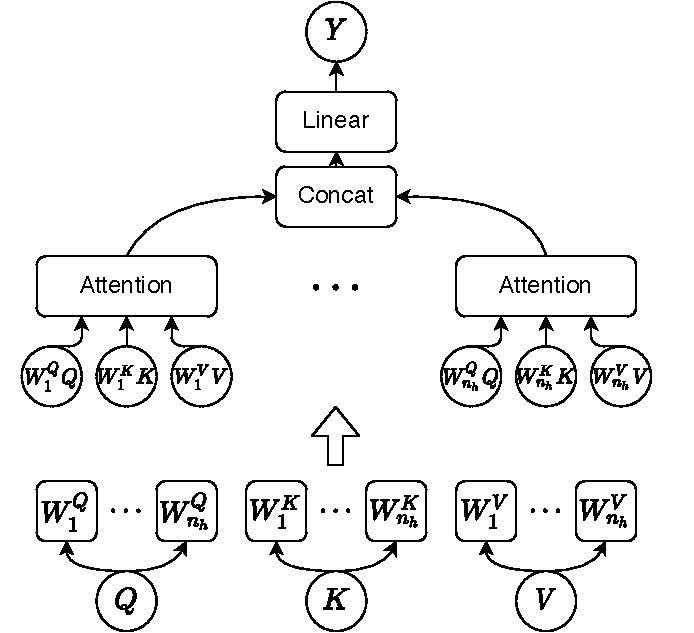
\includegraphics[width=0.8\textwidth]{Figures/multihead-attention.pdf}
\caption{Multi-head attention.
         Adapted from Vaswani et al.~\cite{vaswani2017attention}.}
\label{fig:background:multiheadattn}
\end{figure}

A single attention operator as given by Equation~\ref{eqn:background:attndefn}
would have a theoretical complexity proportional to the query and key
dimension~$c$.
In multi-head attention, we project query, key and value vectors by learned
weights~$W^Q_i \in \mathbb{R}^{c\times c/n_h}$,
$W^K_i \in \mathbb{R}^{c\times c/n_h}$,
and~$W^V_i \in \mathbb{R}^{c\times c/n_h}$, respectively, where~$i$
ranges from~$1$ to~$n_h$.
We then perform the~$n_h$ attention operations on the projected query, key and
value vectors.
Hence, multi-head attention on the projected vectors has the same theoretical
complexity as a single attention operator on the original query, key and value
vectors.
Intuitively, multi-head attention has the advantage that each~$i$th head can
specialize in learning to attend to particular features corresponding to the
affine subspace spanned by columns of the~$i$th projection weight matrix.

We concatenate outputs of the multi-head attention layers and feed the
resulting~$c$-vector into an output linear layer to produce the output~$Y$.
This final concatenation and projection step aggregates information from the
multiple attention heads, for example, to combine information gathered by
different attention heads ``looking at'' different regions of an image.


\subsection{Positional Encoding}

Up until this point in our description of attention, our attention operators
are unable to incorporate positional information, since query and key vectors
interact pairwise with each other.
While recurrent networks have a positional inductive bias, both convolutional
and attention networks are translation equivariant and require injection of
position information to perform position-dependent tasks such as
sequence-to-sequence learning.
Following Gehring et al.'s use of positional encodings for convolutional
sequence-to-sequence networks~\cite{gehring2017convolutional}, in Transformers
Vaswani et al.~\cite{vaswani2017attention} introduced positional encodings to
attention.

Positional encoding means adding to each key vector another vector with encoded
positional information.
Therefore with positional encoding Equation~\ref{eqn:background:attndefn} becomes

\begin{equation}
\mathtt{Attention}_E\big(Q, K, V\big) = \softmax{}\left(\frac{Q(K + E)^\intercal}{\sqrt{c}}\right) V,
\label{eqn:background:posenc-attn}
\end{equation}

\noindent where positional encoding matrix~$E \in \mathbb{R}^{t_2\times c}$ contains a
unique positional encoding~$c$-vector for each of the~$t_2$ elements in our
queried sequence.

We consider positional encodings constructed of learned embeddings, and sinusoidal
positional encodings.
In the case of learned embeddings, the positional encoding matrix~$E$ is
initialized at the beginning of training and updated along with the rest of the
model parameters using backpropagation.
Sinusoidal positional encodings, on the other hand, are not learned and instead
are fixed to a vector of values from a set of sinusoids of varying period
evaluated at the timestep, or sequence element,~$t$.
In particular,

\begin{equation}
\begin{split}
E_{t, 2i} &= \sin\left(\frac{t}{\tau^{2i/c}}\right) \\
E_{t, 2i + 1} &= \cos\left(\frac{t}{\tau^{2i/c}}\right)
\end{split}
\end{equation}

\noindent where~$\tau$ is a fixed constant, for example Vaswani et al.\ fixed~$\tau$
to~\num{10000}.

% TODO(brendan): attention in VQA and VOS

% \subsection{Sparse Attention}


% \subsection{Transformers}


\section{Fusion}

We refer to a topic specific to multimodal applications as fusion.
Following Lahat et al.'s definition~\cite{Lahat2015MultimodalDF}, multimodal
applications involve observing a single phenomenon using data collected from
multiple distinct sensors.
We refer to the raw stream of data collected from each sensor as a modality.
For example, we could treat a video as a multimodal application by making use
of RGB video frames, extracted optical flow and audio as input.
Autonomous driving also makes use of multimodal fusion to combine information
collected from multiple sensors, including LiDAR, radar, and camera
sensors~\cite{Feng2019DeepMO}.

Multimodal fusion refers to the technique by which information extracted from
these multiple raw data streams is combined.
Using fusion holds the promise of producing superior predictions by leveraging
the complementary information contained in separate data streams.
As an example proposed by Kazakos et al.~\cite{kazakos2019TBN}, consider an
egocentric action recognition system that is given as input a video of a person
at a kitchen sink.
When the sink tap is occluded, the audio signal provides a discriminative cue
for the actions ``turn tap on'' and ``turn tap off''.
On the other hand, video input would be more useful for predicting ``wiping
hands'', which has no discriminative auditory signal.
Hence, in this case multiple sensors provide the multimodal action recognition
system with complementary inputs leading to superior predictions.

Traditional multimodal fusion researcher categorize multimodal fusion
techniques into early and late fusion~\cite{ramachandram2017deepmultimodal}.
Early fusion involves combining modalities at the data level, which proves
challenging particularly for data drawn from sensors that may have different
sampling rates or resolutions.
Late fusion became popular in the early 2000s with the rise of ensemble
classifiers~\cite{kuncheva2004combining}.
Compared with early fusion, late fusion proves easier to implement, while
removing the need to retrain models pretrained on each modality, since late
fusion combines modalities at the prediction level.

Deep learning introduced a third category of multimodal fusion, ``intermediate
fusion'', made possible due to deep learning models' hierarchical
representations~\cite{ramachandram2017deepmultimodal}.
Since deep learning models have many layers, which collectively output a
hierarchical feature representation, deep models offer a flexible method for
performing fusion since representations from different modalities can be fused
at different levels of the representation hierarchy.
In deep multimodal models, separate modality-specific encoders, which could be
for example CNNs or RNNs, first extract representations from each modality
independently.
A ``fusion operator'' then combines the modality-specific representations into
a shared representation.

Fusion operators themselves have varying designs. A na\"ive approach would be to
concatenate the representations from different modalities and feed their
concatenation into a feedforward neural network to make a prediction.
However, this simple concatenation may lead to overfitting, and features
extracted from different modalities may be distributed differently so as to
make taking their affine combination an unfavourable fusion strategy.

In general, the subject of designing fusion operators that form effective
priors for combining modalities for a given task is a topic of active research.
Fusion operators are an important component, for example, in the visual
question answering (VQA)~\cite{fukui2016multimodalCB} and image hashtag
prediction~\cite{durand2020learninguserreps} domains.
Standard fusion operators include elementwise sum and product, and
concatenation.
Examples of research into more complex fusion operators include
MCB~\cite{fukui2016multimodalCB}, MUTAN~\cite{ben2017mutan},
GLU~\cite{dauphin2017languagemodeling} and TIRG~\cite{vo2019composing}.
Designing a search space over multimodal fusion operators for VQA is the topic
of our first article.

% \chapter{PROLOGUE TO FIRST ARTICLE}


\section{Article Details}


\section{Context}


\section{Contributions}


\section{Recent Developments}

% \chapter{GENERALIZED HADAMARD-PRODUCT FUSION OPERATORS \\
         FOR VISUAL QUESTION ANSWERING}


\section{Introduction}

Multimodal applications offer a challenge to model selection in machine
learning, as the interactions between different data modalities (e.g.,~between
video and audio, or between images and questions) may require a complicated
prior in order to accurately capture regularities necessary for downstream tasks.

The particular multimodal application that we consider in this work is that of
visual question-answering~(VQA), i.e., of producing a natural language response
to the combined input consisting of an image and a natural language question
pertaining specifically to that image. In the case of VQA, the complexity of
the task exists in both extracting useful feature representations from the
question and the image, as well as the ``fusion'' of these feature
representations by combining them in order to predict the answer to the
question. In this paper, we focus on the problem of combining feature
representations in the VQA task through models based on a generic ``fusion
operator'' definition.

We illustrate the complexity of model selection for the VQA task by designing a
class of multimodal fusion operators, each of which combines raw question and
visual data streams to predict answers to the given questions based on an
image. We evaluate specific instances of high performing fusion operators
belonging to the same design class.

We evaluate and discuss three multimodal fusion architectural components that
emerge as improving performance as part of the investigation into the general
class of fusion operators:

\begin{enumerate}
        \item The use of a gating mechanism, wherein individual features
                extracted by the fusion operator are turned on or off by a
                multiplicative interaction.

        \item The introduction of distinct nonlinearities between parallel
                components in the fusion operator, which we hypothesize adds a
                performance boost due to an ensembling effect.

        \item The additional introduction of learned nonlinearity in the form
                of a neural network inside the fusion operator, which takes
                features from the bilinear interaction of a pair of question
                and visual feature vectors as input.
\end{enumerate}


\section{Related Work}

\subsection{Model Selection}

We propose that the task of model selection applied to multimodal
problem domains can be improved by using automated architecture search techniques.
Reinforcement learning has been used to conduct automated search for neural
network architectures~\cite{zoph2016neural}, gradient
descent optimizers~\cite{bello2017neural} and activation
functions~\cite{ramachandran2017searching}. Other options for architecture
search include evolutionary optimization~\cite{liu2018hierarchical}, Bayesian
optimization~\cite{malkomes2016bayesian}, and gradient descent-based methods.

We contribute to multimodal model selection by describing a generalized class
of fusion operators that can be used as a design space for many of the
search techniques described above. We enable future research to bypass
the difficult problem of model selection for multimodal applications by using
automated model design techniques that use the search space we describe as a
basis.


\subsection{Fusion Operators}

We focus on multimodal fusion of two modalities, applied to the task of visual
question-answering. We use modality to refer to a raw data stream of
information, as would be presented to an observer from a sensor. In the case of
the VQA application, the first modality is the sentence corresponding to the
asked question. The second modality is the image about which the question is
being asked.

Current research in multimodal fusion for VQA focuses
on performance improvements by approximating a bilinear product between a
feature vector~$\q$ extracted from the question, and a feature vector~$\v$
extracted from the
image~\cite{fukui2016multimodalCB, Kim2017, ben2017mutan}.  The feature
vectors $\q$ and $\v$ can be produced by pre-trained feature extraction methods
specific to encoding information from the sentence and image modalities into
vector representations.

In the experimental design of this work, as well as in the work
of~\cite{Kim2017} and~\cite{ben2017mutan}, a pre-trained Residual Network
model~\cite{he2016deep} is used as a feature extractor for the image data
stream, and a pre-trained Skip-Thought
Vectors~\cite{kiros2015skip} model is used to extract features from the
sentence data stream.

In general, we define a fusion operator for the VQA task as a function
$\fusop$, parametrized by~$\thetavec$, of the question feature vector~$\q$ and
the visual feature vector~$\v$. The fusion operator~$\fusop$ computes a vector
output, which is consumed downstream by a function~$g$, e.g.\ a linear layer
followed by a softmax layer, in order to model a probability distribution over
the answer~$y$ conditional on~$\q$ and~$\v$:

\begin{equation}
        p(y \mid \q \,, \v \,; \thetavec) = g(\fusop{(\q \,, \v)}) \,.\
\label{eqn:general-fusion-op}
\end{equation}

The methods of~\cite{fukui2016multimodalCB},
\cite{Kim2017} and~\cite{ben2017mutan} all propose that in the multimodal
application of VQA, the outer product of the feature
vector~$\q$ extracted from the question, with the feature vector~$\v$ extracted
from the image, produces a more expressive feature representation than
straightforward concatenation, element-wise product, or element-wise sum. These previous works design fusion operators based on approximations
to the outer product~$\q \otimes \v$.

The Multimodal Compact Bilinear Pooling (MCB) method
of~\cite{fukui2016multimodalCB} uses the Compact Bilinear Pooling
method of~\cite{gao2016compact} to approximate a bilinear interaction between
$\q$ and $\v$. In the case of MCB, the fusion operator~$\fusop$ consists of
projecting~$\q$ and~$\v$ using Count
Sketch~\cite{Charikar:2002:FFI:646255.684566}, followed by convolution of~$\q$
and~$\v$, which is done efficiently using an element-wise multiplication in
the frequency domain.

The MCB method makes use of the fact that the Count Sketch of the outer
product~$\Psi(\q \otimes \v \,, h \,, s)$, where~$h$ and~$s$ are uniform random
variables as described in~\cite{fukui2016multimodalCB}, is equal in
expectation to the convolution~$\Psi(\q \,, h \,, s) * \Psi(\v \,, h \,, s)$ of
the question and visual feature representations,
i.e.,
$E[\Psi(\q \otimes \v \,, h \,, s)] = E[\Psi(\q \,, h \,, s) * \Psi(\v \,, h \,, s)]$.
However, since this expectation is intractable to
compute,~\cite{Kim2017} proposes a fusion operator based on the Hadamard
(element-wise) product.

The fusion operator in~\cite{Kim2017}, the Multimodal Low-rank Bilinear
Attention Networks~(MLB), uses the Hadamard product coupled with projections
of~$\q$ and~$\v$ with learned weight matrices~$W_\q$ and~$W_\v$, in order to
make a low-rank approximation to the general outer product~$\q \otimes \v$. The
projected vectors are multiplied by a third weight matrix~$W_{\z}$, such that
the fusion operator in the case of~MLB
is~$\fusop{(\q \,, \v)} = {W_{\z}}^\intercal{} ({W_\q}^\intercal{} \q \odot {W_\v}^\intercal{} \v)$,
where~$\odot$ denotes the Hadamard product. Combined, the weight
matrices~$W_\q$, $W_\v$ and~$W_{\z}$ approximate the general weight tensor~$\T$
corresponding to the bilinear interaction between~$\q$ and~$\v$ in the special
case where~$\T$ is of low rank. The idea of using a constrained-rank weight
tensor in the outer product~$\q \otimes \v$ is the same idea used in the MUTAN
fusion operator of~\cite{ben2017mutan}, which generalizes MLB by allowing the
bilinear interaction tensor between~$\q$ and~$\v$ to be of rank $R$.

MUTAN is a fusion operator that is motivated
in~\cite{ben2017mutan} by the Tucker
decomposition~\cite{kolda2009tensor}, which we discuss in
Section~\ref{sec:tucker}. In Section~\ref{sec:model}, we derive the form of
bilinear interaction used by the MUTAN fusion operator from the definition of
the Tucker decomposition, since we base our fusion operator models on this
derivation as well. The MUTAN fusion operator generalizes the MLB fusion
operator to an interaction tensor of rank~$R$, and therefore is,

\begin{equation}
        \fusop{(\q \,, \v)} = \sum_{r = 1}^R {W^r_\z}^\intercal{} ({W^r_\q}^\intercal{} \q \odot {W^r_\v}^\intercal{} \v) \,.
\label{eqn:mutan-fusop}
\end{equation}


\subsection{Tucker Decomposition}
\label{sec:tucker}

\newcommand{\qtWq}{\q^\intercal{} W_\q{}}
\newcommand{\vtWv}{\v^\intercal{} W_\v{}}
\begin{figure}[!t]
\centering
% NOTE(brendan): Source:
% https://tex.stackexchange.com/questions/29877/need-help-creating-a-3d-cube-from-a-2d-set-of-nodes-in-tikz

\makeatletter

% Standard Values for Parameters
\newcommand{\tikzcuboid@shiftx}{0}
\newcommand{\tikzcuboid@shifty}{0}
\newcommand{\tikzcuboid@dimx}{3}
\newcommand{\tikzcuboid@dimy}{3}
\newcommand{\tikzcuboid@dimz}{3}
\newcommand{\tikzcuboid@scale}{1}
\newcommand{\tikzcuboid@densityx}{1}
\newcommand{\tikzcuboid@densityy}{1}
\newcommand{\tikzcuboid@densityz}{1}
\newcommand{\tikzcuboid@rotation}{0}
\newcommand{\tikzcuboid@anglex}{0}
\newcommand{\tikzcuboid@angley}{90}
\newcommand{\tikzcuboid@anglez}{225}
\newcommand{\tikzcuboid@scalex}{1}
\newcommand{\tikzcuboid@scaley}{1}
\newcommand{\tikzcuboid@scalez}{sqrt(0.5)}
\newcommand{\tikzcuboid@linefront}{black}
\newcommand{\tikzcuboid@linetop}{black}
\newcommand{\tikzcuboid@lineright}{black}
\newcommand{\tikzcuboid@fillfront}{white}
\newcommand{\tikzcuboid@filltop}{white}
\newcommand{\tikzcuboid@fillright}{white}
\newcommand{\tikzcuboid@shaded}{N}
\newcommand{\tikzcuboid@shadecolor}{black}
\newcommand{\tikzcuboid@shadeperc}{25}
\newcommand{\tikzcuboid@emphedge}{N}
\newcommand{\tikzcuboid@emphstyle}{thick}
\newcommand{\foreachsteppingx}{%
\ifthenelse{\equal{\dimx}{1}}
    {\foreach \x in {\steppingx,...,\dimx}}
    {\foreach \x in {\steppingx,\secondx,...,\dimx}}
}
\newcommand{\foreachsteppingy}{%
\ifthenelse{\equal{\dimy}{1}}
    {\foreach \y in {\steppingy,...,\dimy}}
    {\foreach \y in {\steppingy,\secondy,...,\dimy}}
}
\newcommand{\foreachsteppingz}{%
\ifthenelse{\equal{\dimz}{1}}
    {\foreach \z in {\steppingz,...,\dimz}}
    {\foreach \z in {\steppingz,\secondz,...,\dimz}}
}

% Definition of Keys
\define@key{tikzcuboid}{shiftx}[\tikzcuboid@shiftx]{\renewcommand{\tikzcuboid@shiftx}{#1}}
\define@key{tikzcuboid}{shifty}[\tikzcuboid@shifty]{\renewcommand{\tikzcuboid@shifty}{#1}}
\define@key{tikzcuboid}{dimx}[\tikzcuboid@dimx]{\renewcommand{\tikzcuboid@dimx}{#1}}
\define@key{tikzcuboid}{dimy}[\tikzcuboid@dimy]{\renewcommand{\tikzcuboid@dimy}{#1}}
\define@key{tikzcuboid}{dimz}[\tikzcuboid@dimz]{\renewcommand{\tikzcuboid@dimz}{#1}}
\define@key{tikzcuboid}{scale}[\tikzcuboid@scale]{\renewcommand{\tikzcuboid@scale}{#1}}
\define@key{tikzcuboid}{densityx}[\tikzcuboid@densityx]{\renewcommand{\tikzcuboid@densityx}{#1}}
\define@key{tikzcuboid}{densityy}[\tikzcuboid@densityy]{\renewcommand{\tikzcuboid@densityy}{#1}}
\define@key{tikzcuboid}{densityz}[\tikzcuboid@densityz]{\renewcommand{\tikzcuboid@densityz}{#1}}
\define@key{tikzcuboid}{rotation}[\tikzcuboid@rotation]{\renewcommand{\tikzcuboid@rotation}{#1}}
\define@key{tikzcuboid}{anglex}[\tikzcuboid@anglex]{\renewcommand{\tikzcuboid@anglex}{#1}}
\define@key{tikzcuboid}{angley}[\tikzcuboid@angley]{\renewcommand{\tikzcuboid@angley}{#1}}
\define@key{tikzcuboid}{anglez}[\tikzcuboid@anglez]{\renewcommand{\tikzcuboid@anglez}{#1}}
\define@key{tikzcuboid}{scalex}[\tikzcuboid@scalex]{\renewcommand{\tikzcuboid@scalex}{#1}}
\define@key{tikzcuboid}{scaley}[\tikzcuboid@scaley]{\renewcommand{\tikzcuboid@scaley}{#1}}
\define@key{tikzcuboid}{scalez}[\tikzcuboid@scalez]{\renewcommand{\tikzcuboid@scalez}{#1}}
\define@key{tikzcuboid}{linefront}[\tikzcuboid@linefront]{\renewcommand{\tikzcuboid@linefront}{#1}}
\define@key{tikzcuboid}{linetop}[\tikzcuboid@linetop]{\renewcommand{\tikzcuboid@linetop}{#1}}
\define@key{tikzcuboid}{lineright}[\tikzcuboid@lineright]{\renewcommand{\tikzcuboid@lineright}{#1}}
\define@key{tikzcuboid}{fillfront}[\tikzcuboid@fillfront]{\renewcommand{\tikzcuboid@fillfront}{#1}}
\define@key{tikzcuboid}{filltop}[\tikzcuboid@filltop]{\renewcommand{\tikzcuboid@filltop}{#1}}
\define@key{tikzcuboid}{fillright}[\tikzcuboid@fillright]{\renewcommand{\tikzcuboid@fillright}{#1}}
\define@key{tikzcuboid}{shaded}[\tikzcuboid@shaded]{\renewcommand{\tikzcuboid@shaded}{#1}}
\define@key{tikzcuboid}{shadecolor}[\tikzcuboid@shadecolor]{\renewcommand{\tikzcuboid@shadecolor}{#1}}
\define@key{tikzcuboid}{shadeperc}[\tikzcuboid@shadeperc]{\renewcommand{\tikzcuboid@shadeperc}{#1}}
\define@key{tikzcuboid}{emphedge}[\tikzcuboid@emphedge]{\renewcommand{\tikzcuboid@emphedge}{#1}}
\define@key{tikzcuboid}{emphstyle}[\tikzcuboid@emphstyle]{\renewcommand{\tikzcuboid@emphstyle}{#1}}
% Commands
\newcommand{\tikzcuboid}[1]{
    \setkeys{tikzcuboid}{#1} % Process Keys passed to command
    \pgfmathsetmacro{\vectorxx}{\tikzcuboid@scalex*cos(\tikzcuboid@anglex)}
    \pgfmathsetmacro{\vectorxy}{\tikzcuboid@scalex*sin(\tikzcuboid@anglex)}
    \pgfmathsetmacro{\vectoryx}{\tikzcuboid@scaley*cos(\tikzcuboid@angley)}
    \pgfmathsetmacro{\vectoryy}{\tikzcuboid@scaley*sin(\tikzcuboid@angley)}
    \pgfmathsetmacro{\vectorzx}{\tikzcuboid@scalez*cos(\tikzcuboid@anglez)}
    \pgfmathsetmacro{\vectorzy}{\tikzcuboid@scalez*sin(\tikzcuboid@anglez)}
    \begin{scope}[xshift=\tikzcuboid@shiftx, yshift=\tikzcuboid@shifty, scale=\tikzcuboid@scale, rotate=\tikzcuboid@rotation, x={(\vectorxx,\vectorxy)}, y={(\vectoryx,\vectoryy)}, z={(\vectorzx,\vectorzy)}]
    \pgfmathsetmacro{\steppingx}{1/\tikzcuboid@densityx}
    \pgfmathsetmacro{\steppingy}{1/\tikzcuboid@densityy}
    \pgfmathsetmacro{\steppingz}{1/\tikzcuboid@densityz}
    \newcommand{\dimx}{\tikzcuboid@dimx}
    \newcommand{\dimy}{\tikzcuboid@dimy}
    \newcommand{\dimz}{\tikzcuboid@dimz}
    \pgfmathsetmacro{\secondx}{2*\steppingx}
    \pgfmathsetmacro{\secondy}{2*\steppingy}
    \pgfmathsetmacro{\secondz}{2*\steppingz}
    \foreachsteppingx
    {
        \foreachsteppingy
        {   \pgfmathsetmacro{\lowx}{(\x-\steppingx)}
            \pgfmathsetmacro{\lowy}{(\y-\steppingy)}
            \filldraw[fill=\tikzcuboid@fillfront,draw=\tikzcuboid@linefront] (\lowx,\lowy,\dimz) -- (\lowx,\y,\dimz) -- (\x,\y,\dimz) -- (\x,\lowy,\dimz) -- cycle;

        }
    }
    \foreachsteppingx
    {
        \foreachsteppingz
        {   \pgfmathsetmacro{\lowx}{(\x-\steppingx)}
            \pgfmathsetmacro{\lowz}{(\z-\steppingz)}
            \filldraw[fill=\tikzcuboid@filltop,draw=\tikzcuboid@linetop] (\lowx,\dimy,\lowz) -- (\lowx,\dimy,\z) -- (\x,\dimy,\z) -- (\x,\dimy,\lowz) -- cycle;
        }
    }
    \foreachsteppingy
    {
        \foreachsteppingz
        {   \pgfmathsetmacro{\lowy}{(\y-\steppingy)}
            \pgfmathsetmacro{\lowz}{(\z-\steppingz)}
            \filldraw[fill=\tikzcuboid@fillright,draw=\tikzcuboid@lineright] (\dimx,\lowy,\lowz) -- (\dimx,\lowy,\z) -- (\dimx,\y,\z) -- (\dimx,\y,\lowz) -- cycle;
        }
    }
    \ifthenelse{\equal{\tikzcuboid@emphedge}{Y}}%
        {\draw[\tikzcuboid@emphstyle](0,\dimy,0) -- (\dimx,\dimy,0) -- (\dimx,\dimy,\dimz) -- (0,\dimy,\dimz) -- cycle;%
        \draw[\tikzcuboid@emphstyle] (0,0,\dimz) -- (0,\dimy,\dimz) -- (\dimx,\dimy,\dimz) -- (\dimx,0,\dimz) -- cycle;%
        \draw[\tikzcuboid@emphstyle](\dimx,0,0) -- (\dimx,\dimy,0) -- (\dimx,\dimy,\dimz) -- (\dimx,0,\dimz) -- cycle;%
        }%
        {}
    \end{scope}
}

\newcommand{\qvectikzdim}{5}
\newcommand{\vvectikzdim}{4}
\newcommand{\cuboidscale}{0.35}


\begin{tikzpicture}
        % NOTE(brendan): Tc
        \tikzcuboid{%
            shiftx=0cm,%
            shifty=0cm,%
            scale=\cuboidscale,%
            rotation=0,%
            densityx=1,%
            densityy=1,%
            densityz=1,%
            dimx=\qvectikzdim,%
            dimy=\vvectikzdim,%
            dimz=3,%
            linefront=black,%
            linetop=black,%
            lineright=black,%
            fillfront=red!50,%
            filltop=green!50,%
            fillright=blue!50,%
            anglex=180,%
            angley=90,%
            anglez=225,%
            scalex=1,%
            scaley=0.8,%
            scalez=0.6,%
            emphedge=N,%
        }

        % NOTE(brendan):
        \tikzcuboid{%
            shiftx=2.0cm,%
            shifty=0cm,%
            scale=\cuboidscale,%
            rotation=0,%
            densityx=1,%
            densityy=1,%
            densityz=1,%
            dimx=1,%
            dimy=\vvectikzdim,%
            dimz=3,%
            linefront=black,%
            linetop=black,%
            lineright=black,%
            fillfront=red!50,%
            filltop=green!50,%
            fillright=blue!50,%
            anglex=180,%
            angley=90,%
            anglez=225,%
            scalex=1,%
            scaley=0.8,%
            scalez=0.6,%
            emphedge=N,%
        }

        \tikzcuboid{%
            shiftx=10pt,%
            shifty=-15mm,%
            scale=\cuboidscale,%
            rotation=0,%
            densityx=1,%
            densityy=1,%
            densityz=1,%
            dimx=\qvectikzdim,%
            dimy=1,%
            dimz=1,%
            linefront=black,%
            linetop=black,%
            lineright=black,%
            fillfront=red!50,%
            filltop=red!50,%
            fillright=red!50,%
            anglex=180,%
            angley=90,%
            anglez=225,%
            scalex=1,%
            scaley=0.8,%
            scalez=0.6,%
            emphedge=N,%
        }

        \newcommand{\qbracesize}{10.2ex}
        \newcommand{\vbracesize}{6.8ex}

        \coordinate (qbrace) at (-0.35, -1.77);
        \node at (qbrace) {\makebox[\qbracesize]{\upbracefill}};
        \node at (qbrace) [below] {$t_q$};

        \coordinate (Tcq brace) at (-0.42, -0.18);
        \node at (Tcq brace) {\rotatebox{180}{\makebox[\qbracesize]{\upbracefill}}};
        \node[inner sep=1pt] at (Tcq brace) [above, fill=white, fill opacity=0.8, text opacity=1, yshift=1.1mm] {$t_q$};

        \node (Tc label) at (Tcq brace) [xshift=-3mm, yshift=18mm] {$\T_c$};
        \node (Tcq label) at (Tc label) [xshift=27mm] {$\T_c^\q$};
        \node (vtWv label) at (Tc label) [xshift=45mm] {$\vtWv$};
        \node[inner sep=0pt] (qtWq label) at (Tc label) [yshift=-43mm, xshift=3mm] {$\qtWq$};
        \node (Tcqv label) at (Tc label) [xshift=65mm] {$\T_c^{\q\v}$};

        \newcommand{\Tcvy}{0.56}
        \coordinate (Tcv brace) at (-1.9, \Tcvy);
        \node at (Tcv brace) {\rotatebox{270}{\makebox[\vbracesize]{\upbracefill}}};
        \node at (Tcv brace) [left] {$t_v$};

        \coordinate (Tco brace) at (0.33, 1.05);
        \node at (Tco brace) {\rotatebox{140}{\makebox[2ex]{\upbracefill}}};
        \node at (Tco brace) [right, yshift=2.0mm, xshift=-1.0mm] {$t_o$};

        \node at (qbrace) [yshift=10mm] {$\times_1$};

        \tikzcuboid{%
            shiftx=3.8cm,%
            shifty=-7pt,%
            scale=\cuboidscale,%
            rotation=0,%
            densityx=1,%
            densityy=1,%
            densityz=1,%
            dimx=1,%
            dimy=\vvectikzdim,%
            dimz=1,%
            linefront=black,%
            linetop=black,%
            lineright=black,%
            fillfront=blue!50,%
            filltop=blue!50,%
            fillright=blue!50,%
            anglex=180,%
            angley=90,%
            anglez=225,%
            scalex=1,%
            scaley=0.8,%
            scalez=0.6,%
            emphedge=N,%
        }

        \coordinate (vbrace) at (4.1, 0.18);
        \node at (vbrace) {\rotatebox{90}{\makebox[\vbracesize]{\upbracefill}}};
        \node at (vbrace) [right] {$t_v$};

        \draw[->, thick, >= stealth] (0.85, 0.25) -- (1.35, 0.25) {};

        \node at (vbrace) [xshift=-11.5mm, yshift=0mm] {$\times_2$};

        \coordinate (tcqv pos) at (5.7, 0.31);

        \draw[->, thick, >= stealth] (4.63, 0.25) -- (5.13, 0.25) {};

        \tikzcuboid{%
            shiftx=5.76cm,%
            shifty=0.3cm,%
            scale=\cuboidscale,%
            rotation=0,%
            densityx=1,%
            densityy=1,%
            densityz=1,%
            dimx=1,%
            dimy=1,%
            dimz=3,%
            linefront=black,%
            linetop=black,%
            lineright=black,%
            fillfront=red!50,%
            filltop=green!50,%
            fillright=blue!50,%
            anglex=180,%
            angley=90,%
            anglez=225,%
            scalex=1,%
            scaley=0.8,%
            scalez=0.6,%
            emphedge=N,%
        }
\end{tikzpicture}

\caption{A geometric representation of the first two $n$-mode products of the
         right hand side Tucker decomposition of Equation~\ref{eqn:tucker-defn},
         where~$A = \qtWq$ and~$B = \vtWv$, i.e.\ $\T_c \times_1 \qtWq \times_2 \vtWv$.
         From left to right, the vector~$\qtWq$ is first combined with the core
         tensor~$\T_c$ by taking the inner product along the dimension of
         size~$t_q$ between~$\qtWq$ and each of the~$t_v \times t_o$ fibers
         composing~$\T_c$, producing the matrix $\T_c^\q$.  Then,~$\vtWv$ is
         combined with~$\T_c^\q$ by taking the inner product between~$\vtWv$
         and the~$t_o$ columns of~$\T_c^\q$, producing the
         vector~$\T_c^{\q{}\v{}}$.}
\label{fig:n-mode-prod}
\end{figure}

The Tucker decomposition is a form of higher-order principal component
analysis~\cite{kolda2009tensor}, which decomposes a tensor into a series of
three $n$-mode tensor products between a single core tensor~$\T_c$ and three
matrices:

\begin{equation}
        \T \approx \T_c \times_1 \A \times_2 \B \times_3 \C
\label{eqn:tucker-defn}
\end{equation}

In Equation~\ref{eqn:tucker-defn}, the $n$-mode tensor product denoted
by~$\times_n$ is the multiplication of a tensor by a matrix, or by a vector, as
in the case of MUTAN and our own method.

In general, the $n$-mode tensor product of a
tensor~$\T \in \R^{I_1 \times I_2 \times \cdots \times I_N}$ with a
matrix~$W \in \R^{J \times I_n}$ yields a new tensor~$\T \times_n W$ with
size~$\TsizeIn{J}$.

In our special case, where we have an $n$-mode product between~$\T$ and a
vector~$\z$, the size of~$\T \times_n \z$ becomes~$\TsizeIn{1}$. The mode-$n$
``fiber'', referring to the generalization of rows and columns of matrices to
higher-order tensors as defined in~\cite{kolda2009tensor},~$\Tfibre$ of~$\T$
along~$I_n$ becomes a single element resulting from the dot product
of~$\Tfibre$ with~$\z$.

Formally, the element-wise definition of the $n$-mode product between
tensor~$\T$ and vector~$\z$ is:

\begin{equation}
        {\big(\T \times_n \z\big)}_{i_1 \cdots i_{n - 1} i_{n + 1} \cdots i_N} = \sum_{i_n = 1}^{I_n} \T_{i_1 \cdots i_N} z_{i_n} \,,
\label{eqn:tucker-decomp-vec-z}
\end{equation}

\noindent where in Equation~\ref{eqn:tucker-decomp-vec-z}, the dimensionality
of~$\T \times_n \z$ is reduced to~$N - 1$ by summing over the~$n$th dimension.
The $n$-mode product is depicted in Figure~\ref{fig:n-mode-prod}.

In Section~\ref{sec:model}, we use the definition of the Tucker decomposition
from Equation~\ref{eqn:tucker-defn}, along with the definition of the $n$-mode
product for the special case of multiplication between a tensor and a vector,
in order to derive the MUTAN fusion operator of Equation~\ref{eqn:mutan-fusop},
and to further generalize the derived fusion operator to include Feature Gating
and Nonlinearity Ensembling.


\section{Methods}

In this section, we present the methods used to
derive a generalization of bilinear fusion operators for the combination of two
feature vectors in multimodal applications. We sub-divide our methods into the
data and model sub-categories of the machine learning process. We first discuss
the data used in our experiments, followed by discussion of the fusion operator
model and how we generalized the model into a class of fusion operators over
which we instantiated and evaluated a range of specific instances.
% TODO(brendan): The inference and criticism sections might only make sense if
% explaining the original RL fusion operator search idea?


\subsection{Data}

The VQA~1.0 dataset~\cite{VQA} is a dataset of ``free-form and open-ended
Visual Question Answering (VQA)''. The VQA task is to give an open-ended
natural language reponse to an input consisting of a natural language question
and an image. In VQA~1.0, there are~\num{23234} unique one-word answers for
real images, and therefore the model's outputs can be represented as a multiple
choice over these answers. In practice, we limit the number of choices to the
top~\num{2000} most common answers in the training dataset.

The VQA~1.0 real images dataset consists of~\num{204}K images from the MSCOCO
dataset~\cite{kolda2009tensor},~\num{614}K questions, and~\num{6}M answers (ten
answers per question). The dataset is separated into a~$2/1/2$
training/validation/test split by the VQA~1.0 authors.

It is known that due to the data collection methodology of the VQA~1.0 dataset,
there exists an imbalance in the dataset that allows questions to be answered
with high accuracy without taking the image into
account; this is remedied with VQA~2.0~\cite{goyal2017making}, which balances the answers to each
question, so that the best scores on the VQA~2.0 dataset are not possible using
language priors alone.

The balancing of VQA~2.0 is due to the addition of complementary images, wherein
for a given image and question pair~$(I, Q)$ with answer~$A$, a complementary
image~$I'$ is found that is similar in appearance, but has a different answer~$A'$ to the
question. The new example~$(I', Q, A')$ is then added to the dataset. VQA~2.0
includes 195K, 93K, and 191K complementary images in the training, validation, and test
sets, respectively. In total, the VQA~2.0 dataset has 443K training, 214K validation, and
453K test (image, question) pairs.

The increased difficulty of the VQA~2.0 dataset with regards to emphasizing the
importance of the combination of visual and question features creates a larger
gap between relatively strong and weak fusion operators, i.e., the performance
gap between strong and weak fusion operators increases when moving from VQA~1.0
to VQA~2.0, even when the absolute performance decreases for
both models under consideration~\cite{goyal2017making}. Therefore, we evaluate
our proposed fusion operators on VQA~2.0.
% TODO(brendan): Experiments using VQA 2.0.


\subsection{Model}
\label{sec:model}

\begin{figure*}[!t]
\centering
% NOTE(brendan): Source:
% https://tex.stackexchange.com/questions/29877/need-help-creating-a-3d-cube-from-a-2d-set-of-nodes-in-tikz

\makeatletter

% Standard Values for Parameters
\newcommand{\tikzcuboid@shiftx}{0}
\newcommand{\tikzcuboid@shifty}{0}
\newcommand{\tikzcuboid@dimx}{3}
\newcommand{\tikzcuboid@dimy}{3}
\newcommand{\tikzcuboid@dimz}{3}
\newcommand{\tikzcuboid@scale}{1}
\newcommand{\tikzcuboid@densityx}{1}
\newcommand{\tikzcuboid@densityy}{1}
\newcommand{\tikzcuboid@densityz}{1}
\newcommand{\tikzcuboid@rotation}{0}
\newcommand{\tikzcuboid@anglex}{0}
\newcommand{\tikzcuboid@angley}{90}
\newcommand{\tikzcuboid@anglez}{225}
\newcommand{\tikzcuboid@scalex}{1}
\newcommand{\tikzcuboid@scaley}{1}
\newcommand{\tikzcuboid@scalez}{sqrt(0.5)}
\newcommand{\tikzcuboid@linefront}{black}
\newcommand{\tikzcuboid@linetop}{black}
\newcommand{\tikzcuboid@lineright}{black}
\newcommand{\tikzcuboid@fillfront}{white}
\newcommand{\tikzcuboid@filltop}{white}
\newcommand{\tikzcuboid@fillright}{white}
\newcommand{\tikzcuboid@shaded}{N}
\newcommand{\tikzcuboid@shadecolor}{black}
\newcommand{\tikzcuboid@shadeperc}{25}
\newcommand{\tikzcuboid@emphedge}{N}
\newcommand{\tikzcuboid@emphstyle}{thick}
\newcommand{\foreachsteppingx}{%
\ifthenelse{\equal{\dimx}{1}}
    {\foreach \x in {\steppingx,...,\dimx}}
    {\foreach \x in {\steppingx,\secondx,...,\dimx}}
}
\newcommand{\foreachsteppingy}{%
\ifthenelse{\equal{\dimy}{1}}
    {\foreach \y in {\steppingy,...,\dimy}}
    {\foreach \y in {\steppingy,\secondy,...,\dimy}}
}
\newcommand{\foreachsteppingz}{%
\ifthenelse{\equal{\dimz}{1}}
    {\foreach \z in {\steppingz,...,\dimz}}
    {\foreach \z in {\steppingz,\secondz,...,\dimz}}
}

% Definition of Keys
\define@key{tikzcuboid}{shiftx}[\tikzcuboid@shiftx]{\renewcommand{\tikzcuboid@shiftx}{#1}}
\define@key{tikzcuboid}{shifty}[\tikzcuboid@shifty]{\renewcommand{\tikzcuboid@shifty}{#1}}
\define@key{tikzcuboid}{dimx}[\tikzcuboid@dimx]{\renewcommand{\tikzcuboid@dimx}{#1}}
\define@key{tikzcuboid}{dimy}[\tikzcuboid@dimy]{\renewcommand{\tikzcuboid@dimy}{#1}}
\define@key{tikzcuboid}{dimz}[\tikzcuboid@dimz]{\renewcommand{\tikzcuboid@dimz}{#1}}
\define@key{tikzcuboid}{scale}[\tikzcuboid@scale]{\renewcommand{\tikzcuboid@scale}{#1}}
\define@key{tikzcuboid}{densityx}[\tikzcuboid@densityx]{\renewcommand{\tikzcuboid@densityx}{#1}}
\define@key{tikzcuboid}{densityy}[\tikzcuboid@densityy]{\renewcommand{\tikzcuboid@densityy}{#1}}
\define@key{tikzcuboid}{densityz}[\tikzcuboid@densityz]{\renewcommand{\tikzcuboid@densityz}{#1}}
\define@key{tikzcuboid}{rotation}[\tikzcuboid@rotation]{\renewcommand{\tikzcuboid@rotation}{#1}}
\define@key{tikzcuboid}{anglex}[\tikzcuboid@anglex]{\renewcommand{\tikzcuboid@anglex}{#1}}
\define@key{tikzcuboid}{angley}[\tikzcuboid@angley]{\renewcommand{\tikzcuboid@angley}{#1}}
\define@key{tikzcuboid}{anglez}[\tikzcuboid@anglez]{\renewcommand{\tikzcuboid@anglez}{#1}}
\define@key{tikzcuboid}{scalex}[\tikzcuboid@scalex]{\renewcommand{\tikzcuboid@scalex}{#1}}
\define@key{tikzcuboid}{scaley}[\tikzcuboid@scaley]{\renewcommand{\tikzcuboid@scaley}{#1}}
\define@key{tikzcuboid}{scalez}[\tikzcuboid@scalez]{\renewcommand{\tikzcuboid@scalez}{#1}}
\define@key{tikzcuboid}{linefront}[\tikzcuboid@linefront]{\renewcommand{\tikzcuboid@linefront}{#1}}
\define@key{tikzcuboid}{linetop}[\tikzcuboid@linetop]{\renewcommand{\tikzcuboid@linetop}{#1}}
\define@key{tikzcuboid}{lineright}[\tikzcuboid@lineright]{\renewcommand{\tikzcuboid@lineright}{#1}}
\define@key{tikzcuboid}{fillfront}[\tikzcuboid@fillfront]{\renewcommand{\tikzcuboid@fillfront}{#1}}
\define@key{tikzcuboid}{filltop}[\tikzcuboid@filltop]{\renewcommand{\tikzcuboid@filltop}{#1}}
\define@key{tikzcuboid}{fillright}[\tikzcuboid@fillright]{\renewcommand{\tikzcuboid@fillright}{#1}}
\define@key{tikzcuboid}{shaded}[\tikzcuboid@shaded]{\renewcommand{\tikzcuboid@shaded}{#1}}
\define@key{tikzcuboid}{shadecolor}[\tikzcuboid@shadecolor]{\renewcommand{\tikzcuboid@shadecolor}{#1}}
\define@key{tikzcuboid}{shadeperc}[\tikzcuboid@shadeperc]{\renewcommand{\tikzcuboid@shadeperc}{#1}}
\define@key{tikzcuboid}{emphedge}[\tikzcuboid@emphedge]{\renewcommand{\tikzcuboid@emphedge}{#1}}
\define@key{tikzcuboid}{emphstyle}[\tikzcuboid@emphstyle]{\renewcommand{\tikzcuboid@emphstyle}{#1}}
% Commands
\newcommand{\tikzcuboid}[1]{
    \setkeys{tikzcuboid}{#1} % Process Keys passed to command
    \pgfmathsetmacro{\vectorxx}{\tikzcuboid@scalex*cos(\tikzcuboid@anglex)}
    \pgfmathsetmacro{\vectorxy}{\tikzcuboid@scalex*sin(\tikzcuboid@anglex)}
    \pgfmathsetmacro{\vectoryx}{\tikzcuboid@scaley*cos(\tikzcuboid@angley)}
    \pgfmathsetmacro{\vectoryy}{\tikzcuboid@scaley*sin(\tikzcuboid@angley)}
    \pgfmathsetmacro{\vectorzx}{\tikzcuboid@scalez*cos(\tikzcuboid@anglez)}
    \pgfmathsetmacro{\vectorzy}{\tikzcuboid@scalez*sin(\tikzcuboid@anglez)}
    \begin{scope}[xshift=\tikzcuboid@shiftx, yshift=\tikzcuboid@shifty, scale=\tikzcuboid@scale, rotate=\tikzcuboid@rotation, x={(\vectorxx,\vectorxy)}, y={(\vectoryx,\vectoryy)}, z={(\vectorzx,\vectorzy)}]
    \pgfmathsetmacro{\steppingx}{1/\tikzcuboid@densityx}
    \pgfmathsetmacro{\steppingy}{1/\tikzcuboid@densityy}
    \pgfmathsetmacro{\steppingz}{1/\tikzcuboid@densityz}
    \newcommand{\dimx}{\tikzcuboid@dimx}
    \newcommand{\dimy}{\tikzcuboid@dimy}
    \newcommand{\dimz}{\tikzcuboid@dimz}
    \pgfmathsetmacro{\secondx}{2*\steppingx}
    \pgfmathsetmacro{\secondy}{2*\steppingy}
    \pgfmathsetmacro{\secondz}{2*\steppingz}
    \foreachsteppingx
    {
        \foreachsteppingy
        {   \pgfmathsetmacro{\lowx}{(\x-\steppingx)}
            \pgfmathsetmacro{\lowy}{(\y-\steppingy)}
            \filldraw[fill=\tikzcuboid@fillfront,draw=\tikzcuboid@linefront] (\lowx,\lowy,\dimz) -- (\lowx,\y,\dimz) -- (\x,\y,\dimz) -- (\x,\lowy,\dimz) -- cycle;

        }
    }
    \foreachsteppingx
    {
        \foreachsteppingz
        {   \pgfmathsetmacro{\lowx}{(\x-\steppingx)}
            \pgfmathsetmacro{\lowz}{(\z-\steppingz)}
            \filldraw[fill=\tikzcuboid@filltop,draw=\tikzcuboid@linetop] (\lowx,\dimy,\lowz) -- (\lowx,\dimy,\z) -- (\x,\dimy,\z) -- (\x,\dimy,\lowz) -- cycle;
        }
    }
    \foreachsteppingy
    {
        \foreachsteppingz
        {   \pgfmathsetmacro{\lowy}{(\y-\steppingy)}
            \pgfmathsetmacro{\lowz}{(\z-\steppingz)}
            \filldraw[fill=\tikzcuboid@fillright,draw=\tikzcuboid@lineright] (\dimx,\lowy,\lowz) -- (\dimx,\lowy,\z) -- (\dimx,\y,\z) -- (\dimx,\y,\lowz) -- cycle;
        }
    }
    \ifthenelse{\equal{\tikzcuboid@emphedge}{Y}}%
        {\draw[\tikzcuboid@emphstyle](0,\dimy,0) -- (\dimx,\dimy,0) -- (\dimx,\dimy,\dimz) -- (0,\dimy,\dimz) -- cycle;%
        \draw[\tikzcuboid@emphstyle] (0,0,\dimz) -- (0,\dimy,\dimz) -- (\dimx,\dimy,\dimz) -- (\dimx,0,\dimz) -- cycle;%
        \draw[\tikzcuboid@emphstyle](\dimx,0,0) -- (\dimx,\dimy,0) -- (\dimx,\dimy,\dimz) -- (\dimx,0,\dimz) -- cycle;%
        }%
        {}
    \end{scope}
}

\newcommand{\qvectikzdim}{5}
\newcommand{\vvectikzdim}{4}
\newcommand{\cuboidscale}{0.35}


\newcommand{\outveccuboid}[2]{%
        \tikzcuboid{%
            shiftx=#1,%
            shifty=#2,%
            scale=\cuboidscale,%
            rotation=0,%
            densityx=1,%
            densityy=1,%
            densityz=1,%
            dimx=1,%
            dimy=1,%
            dimz=3,%
            linefront=black,%
            linetop=black,%
            lineright=black,%
            fillfront=red!50,%
            filltop=green!50,%
            fillright=blue!50,%
            anglex=180,%
            angley=90,%
            anglez=225,%
            scalex=1,%
            scaley=0.8,%
            scalez=0.6,%
            emphedge=N,%
        }
}

\begin{tikzpicture}
        [hadamard/.style={circle,
                          inner sep=0pt,
                          minimum size=6mm,
                          thick,
                          draw=blue!75,
                          fill=blue!20},
         oplussty/.style={circle,
                          inner sep=0pt,
                          minimum size=6mm,
                          thick,
                          draw=cyan!80,
                          fill=cyan!50},
         pre/.style={<-, shorten <= 1pt, >=stealth, semithick},
         post/.style={->, shorten >= 1pt, >=stealth, semithick},
         sumsty/.style={circle,
                        inner sep=0pt,
                        minimum size=6mm,
                        thick,
                        draw=orange!80,
                        fill=orange!50}]

        % Nr
        \newcommand{\nposx}{0.5mm}
        \newcommand{\nposy}{0cm}

        \newcommand{\mposx}{2.15cm}
        \newcommand{\mposy}{-1.0cm}

        \coordinate (mcoord) at (\mposx, \mposy);
        \coordinate (ncoord) at (\nposx, \nposy);

        \coordinate (mtopleft) at (\mposx -1.9cm, \mposy + 0.25cm);
        \coordinate (mbottomright) at (\mposx + 0.5cm, \mposy - 1.5cm);
        \coordinate (ntopleft) at (\nposx -2.0cm, \nposy + 1.15cm);
        \coordinate (nbottomright) at (\nposx + 0.5cm, \nposy - 0.4cm);

        \newcommand{\qtopcolour}{green}
        \newcommand{\qcolourright}{blue}
        \newcommand{\vtopcolour}{green}
        \newcommand{\vcolourfront}{red}
        \tikzcuboid{%
            shiftx=\nposx,%
            shifty=\nposy,%
            scale=\cuboidscale,%
            rotation=0,%
            densityx=1,%
            densityy=1,%
            densityz=1,%
            dimx=1,%
            dimy=\vvectikzdim,%
            dimz=3,%
            linefront=black,%
            linetop=black,%
            lineright=black,%
            fillfront=\vcolourfront!50,%
            filltop=\vtopcolour!50,%
            fillright=blue!50,%
            anglex=180,%
            angley=90,%
            anglez=225,%
            scalex=1,%
            scaley=0.8,%
            scalez=0.6,%
            emphedge=N,%
        }

        \tikzcuboid{%
            shiftx=\mposx,%
            shifty=\mposy,%
            scale=\cuboidscale,%
            rotation=0,%
            densityx=1,%
            densityy=1,%
            densityz=1,%
            dimx=\qvectikzdim,%
            dimy=1,%
            dimz=3,%
            linefront=black,%
            linetop=black,%
            lineright=black,%
            fillfront=red!50,%
            filltop=\qtopcolour!50,%
            fillright=\qcolourright!50,%
            anglex=180,%
            angley=90,%
            anglez=225,%
            scalex=1,%
            scaley=0.8,%
            scalez=0.6,%
            emphedge=N,%
        }

        \newcommand{\vposx}{\nposx - 1.25cm}
        \newcommand{\vposy}{\nposy - 0.24cm}
        \tikzcuboid{%
            shiftx=\vposx,%
            shifty=\vposy,%
            scale=\cuboidscale,%
            rotation=0,%
            densityx=1,%
            densityy=1,%
            densityz=1,%
            dimx=1,%
            dimy=\vvectikzdim,%
            dimz=1,%
            linefront=black,%
            linetop=black,%
            lineright=black,%
            fillfront=blue!50,%
            filltop=blue!50,%
            fillright=blue!50,%
            anglex=180,%
            angley=90,%
            anglez=225,%
            scalex=1,%
            scaley=0.8,%
            scalez=0.6,%
            emphedge=N,%
        }

        \newcommand{\qposx}{\mposx + 0.35cm}
        \newcommand{\qposy}{\mposy - 1.3cm}
        \tikzcuboid{%
            shiftx=\qposx,%
            shifty=\qposy,%
            scale=\cuboidscale,%
            rotation=0,%
            densityx=1,%
            densityy=1,%
            densityz=1,%
            dimx=\qvectikzdim,%
            dimy=1,%
            dimz=1,%
            linefront=black,%
            linetop=black,%
            lineright=black,%
            fillfront=red!50,%
            filltop=red!50,%
            fillright=red!50,%
            anglex=180,%
            angley=90,%
            anglez=225,%
            scalex=1,%
            scaley=0.8,%
            scalez=0.6,%
            emphedge=N,%
        }

        \node (times1) at (mcoord) [xshift=-4mm, yshift=-7mm] {$\times_1$};
        \node (times2) at (ncoord) [xshift=-7mm, yshift=2.5mm] {$\times_2$};

        \node[hadamard, xshift=-0.5cm, yshift=1.25cm] (mutanhadamard) at (mcoord) {$\odot$}
                edge [pre] ($(mtopleft) + (14.0mm, 0.2cm)$)
                edge [pre] ($(nbottomright) + (0.2cm, 6.5mm)$);

        \node (mrqhadamardnrv) at (mutanhadamard) [xshift=4mm, yshift=7mm] {$M_r\mutanfeat{q} \odot N_r\mutanfeat{v}$}
                edge [pre, shorten <= -2pt] (mutanhadamard);

        \node (Rmany) [right=of mutanhadamard, xshift=0mm, yshift=-9mm] {\rotatebox{90}{\makebox[23ex]{\upbracefill}}};

        \node (Rmanytext) [right=of Rmany, xshift=-11mm, text width=12mm] {Repeat $R$ times};

        \node[matrix] (mutanR) [right=of Rmany, xshift=-8mm]
                {%
                        \node (r1) {};\\[2mm]
                        \node (r2) [xshift=6mm] {};\\[2mm]
                        \node (r3) {};\\
                };

        \node[sumsty] (sum) [right=of mutanR, xshift=-0.5cm] {$\Sigma$}
              edge [pre, out=90, in=90] (r1) {}
              edge [pre, out=180, in=0] (r2) {}
              edge [pre, out=270, in=270] (r3) {};

        \node (tcqv) [right=of sum, xshift=-0.5cm] {} edge [pre] (sum) {};

        \pgfgetlastxy{\XCoord}{\YCoord};
        \outveccuboid{\XCoord + 5mm}{\YCoord}

        \begin{scope}[on background layer]
                \node (Mbackground) [fill=red!10, rounded corners, fit=(mtopleft) (mbottomright)] {};
        \end{scope}

        \begin{scope}[on background layer]
                \node (Nbackground) [fill=blue!10, rounded corners, fit=(ntopleft) (nbottomright)] {};
        \end{scope}

        \node[inner sep=0pt] (qlabel) at (mtopleft) [yshift=-1.5cm, xshift=2mm] {$\mutanfeat{q}$};
        \node[inner sep=1pt] (Mlabel) at (mtopleft)
                [yshift=-2mm, xshift=13mm, fill=white, fill opacity=0.9, text opacity=1] {$M_r$};

        \node[inner sep=0pt] (vlabel) at (ntopleft) [yshift=-0.2cm, xshift=0.15cm] {$\mutanfeat{v}$};
        \node[inner sep=1pt] (Nlabel) at (ntopleft)
                [yshift=-8.5mm, xshift=20mm, fill=white, fill opacity=0.9, text opacity=1] {$N_r$};

        \node[matrix] (legend) at (current bounding box.east) [xshift=3.5cm] {%
                \node[hadamard, label=right:Element-wise multiplication.] {$\odot$};\\[2mm]
                \node[sumsty, label=right: Element-wise sum.] {$\Sigma$};\\[2mm]
                \node[oplussty, label=right: Binary operator~$b$.] {$\binopb$};\\[2mm]
                \node[minimum size=6mm, label={[xshift=1mm]right: $\qtWq$}] {$\mutanfeat{q}$};\\[2mm]
                \node[minimum size=6mm, label={[xshift=1mm]right: $\vtWv$}] {$\mutanfeat{v}$};\\
        };

        \begin{scope}[on background layer]
                \node (r1) [fill=black!10, rounded corners, fit=(legend)] {};
        \end{scope}


        \newcommand{\ourstopleftx}{-1.5cm}
        \newcommand{\ourstoplefty}{-2.5cm}
        \coordinate (ours top left) at (\ourstopleftx, \ourstoplefty);

        \node (q1) [below=of ours top left] {$M_{r}\mutanfeat{q}$};
        \node (v1) [below=of q1] {$N_{r}\mutanfeat{v}$};
        \node[hadamard, xshift=1.5cm] (h1) at ($(q1)!0.5!(v1)$) {$\odot$}
                 edge [pre] node [below] {$f_{\mathrm{rv}}$} (v1) {}
                 edge [pre] node [above, xshift=1mm] {$f_{\mathrm{rq}}$} (q1) {};

        \begin{scope}
                [cnode/.style={draw=black,fill=#1,minimum width=3mm,circle},
                 scale=0.5,
                 shift={($(h1) + (2.0cm, 3.0cm)$)}]
                \newcommand{\layertwoxshift}{2}
                \node at (0,-3.75) {$\vdots$};
                \node at (\layertwoxshift,-3.75) {$\vdots$};
                \foreach \x in {1,...,4}
                {
                        \pgfmathparse{\x<4 ? \x : "n"}
                        \node[cnode=gray!50] (x-\x) at (0,{-\x-div(\x,4)}) {};
                        \node[cnode=gray!50] (p-\x) at (\layertwoxshift,{-\x-div(\x,4)}) {};
                }
                \foreach \x in {1,...,4}
                {   \foreach \y in {1,...,4}
                {   \draw (x-\x) -- (p-\y);
                }
                }

                \draw[post] (h1) -- (x-3);
        \end{scope}

        \node (oursRmany) [right=of p-1, xshift=-9mm, yshift=-10mm] {\rotatebox{90}{\makebox[14ex]{\upbracefill}}};
        \node (oursRmanytext) [right=of oursRmany, xshift=-11mm, text width=12mm] {Repeat $R$ times};

        \pgfgetlastxy{\XCoord}{\YCoord};
        \foreach \y/\ytext in {0cm/0, -0.75cm/1, -1.5cm/2, -2.25cm/3}
        {
                \node (outvec\ytext) at (\XCoord + 25mm, \YCoord + 11mm + \y) {}
                        edge [pre, out=180, in=0, shorten <= 8pt, shorten >= -5pt] (oursRmanytext) {};
                \outveccuboid{\XCoord + 25mm}{\YCoord + 10mm + \y}
        }

        \coordinate (outvec01mid) at ($(outvec0)!0.5!(outvec1)$);
        \newcommand{\oplusedgexshift}{3pt};
        \newcommand{\oplusinangleLO}{145}
        \newcommand{\oplusinangleHI}{215}
        \node[oplussty, label={[xshift=0.5mm, yshift=0mm]center:$\binop_1$}]
                (oplus1) [right=of outvec01mid] {}
                edge [pre, out=\oplusinangleLO, in=0, shorten >= \oplusedgexshift] (outvec0) {}
                edge [pre, out=\oplusinangleHI, in=0, shorten >= \oplusedgexshift] (outvec1) {};

        \coordinate (outvec23mid) at ($(outvec2)!0.5!(outvec3)$);
        \node[oplussty, label={[xshift=0.5mm, yshift=0mm]center:$\binop_2$}]
                (oplus2) [right=of outvec23mid] {}
                edge [pre, out=\oplusinangleLO, in=0, shorten >= \oplusedgexshift] (outvec2) {}
                edge [pre, out=\oplusinangleHI, in=0, shorten >= \oplusedgexshift] (outvec3) {};

        \coordinate (oplusmid) at ($(oplus1)!0.5!(oplus2)$);
        \newcommand{\oplusshortenTWO}{0pt};
        \node[oplussty, label={[xshift=0.5mm, yshift=0mm]center:$\binop_2$}]
                (oplus3) [right=of oplusmid] {}
                edge [pre, out=90, in=0, shorten >= \oplusshortenTWO] (oplus1) {}
                edge [pre, out=270, in=0, shorten >= \oplusshortenTWO] (oplus2) {};

        \node (ourstcqv) [right=of oplus3, xshift=-0.5cm] {} edge [pre] (oplus3) {};

        \pgfgetlastxy{\XCoord}{\YCoord};
        \outveccuboid{\XCoord + 5mm}{\YCoord}

        \newcommand{\leftlinexshift}{-2mm}
        \coordinate (left line bottom) at
                ($(current bounding box.south west) + (\leftlinexshift, 0)$);
        \coordinate (left line top) at
                ($(current bounding box.north west) + (\leftlinexshift, 0)$);
        \draw[semithick] (left line bottom) -- (left line top);

        \node[xshift=-3mm, yshift=-20mm, rotate=90]
                (mutan label) at (left line top) {MUTAN};

        \node[xshift=-3mm, yshift=15mm, rotate=90]
                (mutan label) at (left line bottom) {Ours};
\end{tikzpicture}

\caption{A comparison between the MUTAN fusion operator of~\cite{ben2017mutan}
         (top) and our generalized fusion operator (bottom). Both MUTAN and our
         fusion operator take the features~$M_r\mutanfeat{q}$
         and~$N_r\mutanfeat{v}$ as input. MUTAN approximates the Tucker
         decomposition shown in Figure~\ref{fig:n-mode-prod} by constraining
         the bilinear interaction between the vectors~$\mutanfeat{q}$
         and~$\mutanfeat{v}$ to be of rank~$R$.
         Note that while~$\T_c$ in Figure~\ref{fig:n-mode-prod} is a learned
         tensor whose parameters implicitly describe the bilinear interaction
         between~$\mutanfeat{q}$ and~$\mutanfeat{v}$, here the parameters
         of~$M_r$ and~$N_r$ are separate and the bilinear interaction is due to
         the Hadamard product.
         Our fusion operator generalizes MUTAN first by allowing different
         nonlinearities~$f_{rq}$ and~$f_{rv}$ to act on the
         features~$M_r\mutanfeat{q}$ and~$N_r\mutanfeat{v}$. The result is then
         composed with an additional learned nonlinearity in the form of a
         neural network, producing a set of~$R$ output features, as in MUTAN
         after the Hadamard product
         step~$M_r\mutanfeat{q} \odot N_r\mutanfeat{v}$.  In the case of MUTAN,
         the~$R$ output feature vectors are combined by element-wise summation,
         whereas in our fusion operator the~$R$ feature vectors are combined by
         applying a tree of binary operators~$\binopb$, as described by
         Algorithm~\ref{alg:apply-binop-seq}.}
\label{fig:mutan-ours}
\end{figure*}

Following the work of~\cite{Kim2017} and~\cite{ben2017mutan}, we represent the
sentence and visual modalities with extracted feature vectors. We use a
pre-trained Skip-Thought Vectors model~\cite{kiros2015skip}
to extract a ``question vector'' feature representation~$\q$ from a question.
As well, we use a ResNet~\cite{he2016deep} pre-trained on
ImageNet~\cite{russakovsky2015imagenet} to extract a ``visual vector'' feature
representation~$\v$ from an image.

For the purpose of this paper, the Skip-Thought Vectors model and ResNet can
each be thought of as ``black boxes'' used to extract useful feature
representations from sentences and images, respectively. By using this
black-box abstraction, the fusion operators we develop can automatically
benefit from improved feature extraction models without altering the algorithm
presented here.

The Skip-Thought Vectors model extracts a $d_q$ vector from the question, and
the ResNet model extracts a~$d_v \times S \times S$ tensor from the image,
where~$S$ is the pre-pooling spatial dimension of the feature maps produced by
the ResNet.

The MUTAN fusion operator of~\cite{ben2017mutan} and MLB fusion operator
of~\cite{Kim2017} combine the image and sentence feature vectors by
approximating a bilinear interaction between the vectors. The bilinear
interaction is learned, and the output of that interaction is input into a
linear predictive layer, which is in turn fed into a softmax layer that outputs
probabilities over the top~\num{2000} most common answers in the training data.

We generalize the bilinear interaction of MUTAN and MLB such that both MLB and
MUTAN, as well as element-wise multiplication and element-wise addition, can
all be represented in a common form.

We derive our fusion operator as a generalization of the MUTAN fusion operator
by first deriving MUTAN from the definition of the Tucker
decomposition~\cite{kolda2009tensor}, then discussing the generalization of
this expression.  We begin from the definition of the Tucker decomposition
given in Equation~\ref{eqn:tucker-defn}.

In the case of MUTAN, $\A$ in Equation~\ref{eqn:tucker-defn} corresponds to the
vector~$\qtWq \in \R^{1 \times t_q}$, $\B$
is~$\vtWv \in \R^{1 \times t_v}$,
and~$\C$ is~$W_o \in \R^{|A| \times t_o}$, where~$|A|$ is the
dimensionality of the output vector (i.e., the number of answer classes),
and~$t_q$, $t_v$ and~$t_o$ are the respective dimensionalities of the vector
spaces that the question features, image features, and fused question-image
features are projected onto before applying a linear prediction layer~$W_o$.

Therefore, MUTAN is a special case of the Tucker decomposition in
Equation~\ref{eqn:tucker-defn}, as given by Equation~\ref{eqn:tucker-mutan},
where~$\mathbf{y}$ is the prediction output of the fusion operator:

\begin{equation}
        \mathbf{y} = \T_c \times_1
                \qtWq \times_2
                \vtWv \times_3
                W_o
        \label{eqn:tucker-mutan}
\end{equation}

In the following, we derive from the Equation~\ref{eqn:tucker-mutan} form of
MUTAN an expression for MUTAN that can be generalized to a family of fusion
operators, over which a variety of specific instantiations can be chosen and
evaluated.  Throughout the derivation, $\mutanfeat{q}$ is shorthand for
$\qtWq$, and $\mutanfeat{v}$ represents $\vtWv$.

Referring to $\T_c \times_1 \qtWq$ as $\T_c^{\q}$, each element of
the matrix $\T_c^{\q}$ in terms of elements of~$\mutanfeat{q}$ and~$\T_c$ is
$\T_c^{\q}[j, k] = \sum_{i = 1}^{t_q} \T_c[i, j, k] \cdot \mutanfeat{q}[i]$,
which follows from the definition of the $n$-mode tensor product.

Similarly, we expand the elements of the
vector~$\T_c^{\q\v} = \T_c^{\q} \mutanfeat{v}$ in terms of elements
of~$\mutanfeat{q}$ and~$\mutanfeat{v}$, and slices of~$\T_c$.

\begin{align}
\begin{split}
        \T_c^{\q\v}[k] &= \sum_{j = 1}^{t_v} \T_c^{\q}[j, k] \cdot \mutanfeat{v}[j]  \\
                       &= \sum_{j = 1}^{t_v} \biggl(\sum_{i = 1}^{t_q} \T_c[i, j, k] \cdot \mutanfeat{q}[i]\biggr) \cdot \mutanfeat{v}[j]  \\
                       &= {\mutanfeat{q}}^\intercal \T_c[:, :, k] \mutanfeat{v}
\end{split}
\label{eqn:tucker-core-tensor-expanded}
\end{align}

The constraint enforced by~\cite{ben2017mutan} in MUTAN is that each slice of
the core tensor, i.e.,~$\T_c[:, :, k]$, must be of rank~$R$, and therefore a sum
of matrices each given by an outer product of vectors. Therefore,

\begin{equation}
        \T_c[:, :, k] = \sum_{r = 1}^R \m_r^k \otimes \n_r^k
                      = \sum_{r = 1}^R \m_r^k {\n_r^k}^\intercal \,,
\label{eqn:tucker-core-tensor-rank-r}
\end{equation}

\noindent where~$\m_r^k \in \R^{t_q \times 1}$ and~$\n_r^k \in \R^{1 \times t_v}$.
Substituting Equation~\ref{eqn:tucker-core-tensor-rank-r} into the last line of
Equation~\ref{eqn:tucker-core-tensor-expanded} gives:

\begin{align}
\begin{split}
        \T_c^{\q\v}[k] &= {\mutanfeat{q}}^\intercal
                \biggl(\sum_{r = 1}^R \m_r^k {\n_r^k}^\intercal\biggr) \mutanfeat{v}  \\
                     &= \sum_{r = 1}^R \left({\mutanfeat{q}}^\intercal \m_r^k\right)
                                \left({\n_r^k}^\intercal \mutanfeat{v}\right) \,,
\end{split}
\label{eqn:tucker-core-element-wise}
\end{align}

\noindent where each term in the sum is a scalar.
Equation~\ref{eqn:tucker-core-element-wise} states that $\T_c^{\q{}\v{}}$ is the sum
over $r~\in~\{1, \dots, R\}$ of matrix-vector element-wise products
$M_r \mutanfeat{q} \odot N_r \mutanfeat{v}$, i.e.,

\begin{equation}
        \T_c^{\q{}\v{}} =
                \sum_{r = 1}^R M_r \mutanfeat{q} \odot N_r \mutanfeat{v} \,.
\label{eqn:tucker-decomp-hadamard}
\end{equation}

\noindent In Equation~\ref{eqn:tucker-decomp-hadamard}, $M_r \in \R^{t_o \times t_q}$
and~$N_r \in \R^{t_o \times t_v}$ are learned matrices, whose rows are the
vectors $\m_r^k$ and $\n_r^k$, respectively.

We have presented an equivalent form of the MUTAN fusion operator in
Equation~\ref{eqn:tucker-decomp-hadamard}, of which the MLB fusion operator
of~\cite{Kim2017} is a special case where~$R = 1$. In this paper, we propose a
further generalized extension to Equation~\ref{eqn:tucker-decomp-hadamard}, by
allowing the fusion operator to contain the following transformations:

\begin{itemize}
        \item A unique pair of unary activation
                functions~$(f_{rq}, f_{rv})$ that can wrap the individual
                factors before the Hadamard product. We refer to the
                combination of unique pairs of nonlinearities as Nonlinearity
                Ensembling.

        \item A sequence of~$L$ neural network layers~$\phi_l$ composing a
                feedforward neural network module~$\Phi$ that can take the features
                produced by the bilinear
                interaction~$M_r \mutanfeat{q} \odot N_r \mutanfeat{v}$ as
                input, thereby introducing additional nonlinearity into the
                fusion operator.

        \item Skip connections~\cite{he2016deep, srivastava2015training} may
                exist between the inputs to the fusion operator, the outputs of
                any given neural network layer~$\phi_j$ in the fusion operator,
                and the inputs to any other neural network layer~$\phi_k$, or
                the final output of the fusion operator.

        \item The sum over~$R$ terms in
                Equation~\ref{eqn:tucker-decomp-hadamard} is generalized to
                arbitrary binary relations~$\binopb(\cdot \,, \cdot)$. Each
                binary relation~$\binopb$ is associated with a
                set~$\binoppartition$ corresponding to an element of a
                partition of the outputs~$\tuckbranch$ from the~$R$ branches of
                the fusion operator, before those branches are joined.
                $\tuckbranch$ is defined according to
                Equation~\ref{eqn:general-fusion-op-defn}:

                \begin{equation}
                \tuckbranch =
                \Phi_r(f_{rq}{\left(M_r \mutanfeat{q}\right)} \odot f_{rv}{\left(N_r \mutanfeat{v}\right)}) \,.
                \label{eqn:general-fusion-op-defn}
                \end{equation}

                There is also an ordering over the binary operations such
                that~$\binopb$ form a sequence~$\binopseq$, where $B$
                represents the total number of distinct binary operators and is
                equal to the number of subsets in the
                partition~$\binoppartition$.

                The sequence~$\binopseq$ is applied recursively to the
                partitions~$\binoppartB_b \coloneqq \binoppartition$ according
                to Algorithm~\ref{alg:apply-binop-seq}.

                The generalization over binary operators allows for binary
                operations besides addition to be applied to the~$\tuckbranch$
                output from each branch of the fusion operator, and also allows
                definition of precedence rules so that binary operators can be
                applied in a defined order. The fusion operator in
                Equation~\ref{eqn:tucker-decomp-hadamard} is the special case
                of the generalized fusion operator where~$B = 1$,
                $\binop_1 = +$, and~$\binoppartB_1$ is the entire set of branch
                outputs~$\{\tuckbranch\}$.
\end{itemize}

\begin{algorithm}
\begin{algorithmic}[1]
        \Function{ApplyBinOpSequence}
                 {$\binoppartBseq, \binopseq$}
                \State{$v \gets \Call{Identity}{\binop_1}$}
                \ForAll{$b \in \{1, \dots, B\}$}
                        \State{$v_b \gets \Call{Identity}{\binopb}$}
                        \ForAll{$\tuckbranch \in \binoppartB_b$}
                                \State{$v_b \gets v_b \binopb \tuckbranch$}
                        \EndFor{}
                        \State{$v \gets v \binopb v_b$}
                \EndFor{}
                \State{\Return{$v$}}
        \EndFunction{}
\caption{Recursively applies the binary operator sequence~$\binopseq$ to the
        sequence~$\binoppartBseq$ of elements of a partition of the set of
        outputs from each of the~$R$ branches of the generalized fusion
        operator. The~$\textproc{Identity}{(\binop)}$ function returns the
        identity for the binary operator~$\binop$.}
\label{alg:apply-binop-seq}
\end{algorithmic}
\end{algorithm}

% TODO(brendan): Attention part of the model.

Our generalized fusion operator is compared alongside MUTAN in
Figure~\ref{fig:mutan-ours}.


\section{Experiments}
\label{sec:experiments}

In this section, we instantiate specific models based on the generalized fusion
operator described by Algorithm~\ref{alg:apply-binop-seq}. We individually
test the specific extensions for a generalized fusion operator, as described in
Section~\ref{sec:model}. We then demonstrate the degree to which the
extensions' performance gains are complementary.

In all of the following experiments, the Adam
optimizer~\cite{kingma2014adam} is used to train each model with a learning
rate of~$10^{-4}$. The models are trained for~\num{100} epochs. For the validation
set, models with the best validation accuracy are selected. For the test-dev
set, the model parameters used to generate test-dev predictions correspond to
the early-stopping epoch determined from the validation set.

Following the hyperparameter settings of~\cite{ben2017mutan}, the number of
branches used in the fusion operator is~$R = 5$. The dimensionality of the
question vector~$\q$ is the default for uni-skip Skip-Thought Vectors~$d_q =
2400$, while the visual vector~$\v$ is the~$d_v = 2048$ dimensional output of a
ResNet.  Question and visual features are projected into a~$t_q = t_v = 310$
dimensional vector space before being reprojected into a~$t_o = 510$
dimensional vector space where~$\q$ and~$\v$ are combined by Hadamard product.
The batch size used in our experiments is~\num{128}.


\subsection{Nonlinearity Ensembling (NE)}

To test the contribution of using a variety of activation functions per branch
of the fusion operator, we first conducted a grid search over possible
combinations where each~$f_{rq}$ and~$f_{rv}$ was drawn uniformly from the
following set of candidate nonlinearities: identity function, leaky
ReLU~\cite{maas_rectified_nonlinearities},
SeLU~\cite{klambauer2017self}, sigmoid, and tanh. We subsampled the VQA~1.0
dataset and ran a grid search with each run lasting only~\num{5} epochs in
order to quickly observe many combinations of nonlinear activation function
pairs.

From the grid search, we observed the pattern that the stronger nonlinearity
pair combinations used SeLU as the visual vector activation function, while
using a variety of different activation functions on the question vector.
Therefore, to test Nonlinearity Ensembling, we used branches where the visual
vectors always used the SeLU nonlinearity, and the branches used one of each
activation function on the question vector.

We propose that the diversity in the activation function on the question vector
decreases the correlation between the branches, hence improving the ensembling
effect of summing the branches' predictions together.


\subsection{Post-fusion neural networks with skip connections}
% TODO(brendan): Figure with post-fusion NN and skip connections

In order to allow for a nonlinear function to act on the bilinear features
extracted by the Hadamard product between~$M_r\mutanfeat{q}$
and~$N_r\mutanfeat{v}$, we propose adding a neural network~$\Phi_r$ to the
fusion operator. We embed a ``tiny'' neural network in the fusion operator
analogous to how Network in Network~\cite{lin2013network} embeds a tiny neural
network in a convolution.

In our implementation, $\Phi_r$ consists of a sequence of blocks of three
feedforward layers where the activation function for each layer matches that
of~$f_{rq}$.  There is a skip connection from the input, and from every third
layer, to the output.


\subsection{Feature Gating (FG) and Polarity Swap (PS)}
% TODO(brendan): Show a matrix of which features are activated for which types
% of questions.

\begin{figure*}[!t]
\centering
\newcommand{\branchstub}[5]{%
\begin{scope}[yshift=#2]
\node (q#1) {$M_{#5}\mutanfeat{q}$};
\node (v#1) [below=of q#1] {$N_{#5}\mutanfeat{v}$};

\node[hadamard, xshift=2cm] (h#1) at ($(q#1)!0.5!(v#1)$) {$\odot$}
         edge [pre] node [below] {$f_{\mathrm{selu}}$} (v#1) {}
         edge [pre] node [above, xshift=#4] {$f_{\mathrm{#3}}$} (q#1) {};

\node[nn] (nn#1) [right=of h#1] {$\Phi_#5$}
        edge [pre] (h#1) {};
\end{scope}}

\newcommand{\vecelems}[1]{%
        \node [matrix, vecsty]
                (vector#1) [right=of nn#1, xshift=1cm]
                {%
                        \node[rectangle] (vec#1a) {$t_1$};\\
                        \node[rectangle] (vec#1b) {$t_2$};\\[-2mm]
                        \node[rectangle] (vec#1c) [xshift=1mm] {$\vdots$};\\
                        \node[rectangle] (vec#1d) {$t_o$};\\
                };

        \draw [post, shorten >= 3pt, red!80, thick] (nn#1) -- (vector#1);
        \fill[left color=red!80, middle color=red!65, right color=red!50] ($(nn#1)!0.5!(vector#1)$) -- (vector#1.north west) -- (vector#1.south west) -- cycle;
}

\begin{tikzpicture}
        [gate/.style={circle,
                      inner sep=0pt,
                      minimum size=2mm,
                      thick,
                      draw=black,
                      fill=white},
         gateedge/.style={-{Circle[fill=white]},
                          out=0,
                          in=180,
                          shorten >= 3pt,
                          semithick},
         hadamard/.style={circle,
                          inner sep=0pt,
                          minimum size=6mm,
                          thick,
                          draw=blue!75,
                          fill=blue!20},
         nn/.style={rectangle,
                    draw=black!50,
                    fill=black!20,
                    thick,
                    inner sep=0pt,
                    minimum size=6mm},
         pre/.style={<-, shorten <= 1pt, >=stealth, semithick},
         post/.style={->, shorten >= 1pt, >=stealth, semithick},
         sigmoid/.style={circle,
                         inner sep=0pt,
                         minimum size=4mm,
                         thick,
                         draw=black,
                         fill=green!50,
                         draw=green!80},
         sumsty/.style={circle,
                        inner sep=0pt,
                        minimum size=6mm,
                        thick,
                        draw=orange!80,
                        fill=orange!50},
         vecsty/.style={fill=red!50, draw=red!80, very thick}]

        \branchstub{1}{0cm}{tanh}{1mm}{1}
        \branchstub{2}{-2.5cm}{identity}{2mm}{\sigma}

        \branchstub{3}{-5cm}{sigmoid}{2mm}{2}

        \vecelems{1}
        \vecelems{3}

        \node[sigmoid] (sigmoid2)
                [right=of nn2, xshift=-5mm] {$\sigma$}
                edge [pre] (nn2) {}
                edge [gateedge] (vec1a) {}
                edge [gateedge] (vec1b) {}
                edge [gateedge] (vec1d) {}
                edge [gateedge] (vec3a) {}
                edge [gateedge] (vec3b) {}
                edge [gateedge] (vec3d) {};

        \node[sumsty] (sum) [right=of sigmoid2, xshift=2cm] {$\Sigma$}
              edge [pre, out=90, in=0] (vector1) {}
              edge [pre, out=270, in=0] (vector3) {};

        \node (tcqv) [right=of sum] {$\T_c^{\q\v}$}
                edge [pre] (sum) {};

        \node[matrix] (legend) at (current bounding box.east) [xshift=3.5cm] {%
                \node[label=right:Question vector features.] {$\q$};\\[2mm]
                \node[label=right:Image vector features.] {$\v$};\\[2mm]
                \node[hadamard, label=right:Element-wise multiplication.] {$\odot$};\\[2mm]
                \node[nn, label=right:Neural network layers~${(\phi_l)}_r$.] {$\Phi_r$};\\[2mm]
                \node[sigmoid, label=right:Logistic sigmoid nonlinearity.] {$\sigma$};\\[2mm]
                \node[gate, label=right:Scalar multiplication.] {};\\[2mm]
                \node[vecsty, label=right: Elements of~$\tuckbranch \in \mathbb{R}^{t_o}$.] {$t_i$};\\[2mm]
                \node[sumsty, label=right: Element-wise sum.] {$\Sigma$};\\
        };

        \begin{scope}[on background layer]
                \node (r1) [fill=black!10, rounded corners, fit=(legend)] {};
        \end{scope}
\end{tikzpicture}

\caption{An example network using the Feature Gating neural
         network component, where each node represents a computation and
         the arrows represent the forward flow of information. The question and
         image feature vectors~$\q$ and~$\v$ are shared inputs to all branches.
         The~$\Phi_r$ nodes represent post-fusion feedforward neural networks
         with skip connections. The logistic sigmoid node~$\sigma$ squashes
         output features~$\T_\sigma^{\q{}\v{}}$ from~$\Phi_\sigma$ to a vector
         of values in~$(0, 1)$. The output from~$\sigma$ is element-wise
         multiplied with all other~$\tuckbranch$ features from each branch,
         effectively turning on or off each feature channel. The resultant
         gated~$\tuckbranch$ features are summed to become~$\T_c^{\q{}\v{}}$,
         features that are input into a predictive layer to score the most
         common answers to questions from the VQA task.}
\label{fig:feature-gating}
\end{figure*}

Algorithm~\ref{alg:apply-binop-seq} introduces a method of generalizing the sum
operation over fusion operator branch outputs~$\tuckbranch$ to an ordered set
of binary operations. We test two particular instantiations of
Algorithm~\ref{alg:apply-binop-seq} where~$B = 2$, $\binop_1 = +$,
$\binop_2 = \odot$ and $|\binoppartB_2| = 1$, i.e.~$R - 1$ of the branch
outputs~$\tuckbranch$ are summed and then element-wise multiplied by the
remaining branch output.

Assume that the branch output that gets multiplied with the sum of the other
branch outputs is~$\T_R^{\q{}\v{}}$. The output of~$\T_R^{\q{}\v{}}$ is first
squashed by a nonlinearity~$f$ before being multiplied into the sum
over~$\binoppartB_1$.

In the case of our first experiment, the squashing nonlinearity is the logistic
function~$f_\mathrm{sigmoid}$, which independently squashes the
output~$f_\mathrm{sigmoid}(\T_R^{\q{}\v{}})$ into the range~$(0, 1)$. The
effect of multiplying by this squashed output is therefore to turn each feature
on or off, so we refer to the first experiment as Feature Gating.

The squashing nonlinearity used in the second experiment is
tanh~$f_{\tanh}$, which has the effect of
squashing~$f_{\tanh}(\T_R^{\q{}\v{}})$ to the range~$(-1, 1)$. We refer to the
second experiment as Polarity Swap, since negative features can be
conditionally swapped to positive and vice-versa.

Figure~\ref{fig:feature-gating} demonstrates an example instantiated fusion
operator that makes use of the Feature Gating idea, and implements the
Feature Gating experiment described above. In Figure~\ref{fig:feature-gating},
the number of branches is set to~$R = 3$ for clarity, while in the experiments
of Table~\ref{tab:model-ablation}, the models have~$R = 5$ branches.


\section{Results}

In Table~\ref{tab:model-ablation}, we compare performance improvements between
different instantiations of the generalized fusion operator described in
Equation~\ref{eqn:general-fusion-op-defn} and
Algorithm~\ref{alg:apply-binop-seq}, which are discussed in
Section~\ref{sec:experiments}. We use the VQA~1.0 validation set to compare the
effect on the performance of fusion operators of adding Nonlinearity
Ensembling, as well as Feature Gating and Polarity Swap, independently. We
chose to first investigate these static components of the fusion operator
design before fixing them while investigating possible post-fusion neural
networks.  Since the neural network is a learned component of the architecture,
it has to adapt to the static components during training, and hence the optimal
hyperparameters of the neural network may vary depending on the choice of
static components in the model.

\begin{table}[!t]
\centering
\caption{An ablation study on Nonlinearity Ensembling, Feature Gating, and
         Polarity Swap.}
\begin{tabular}{rc}
\textbf{Model} & \textbf{VQA 1.0 val} \\
\midrule
MUTAN~\cite{ben2017mutan} & 61.54 \\
\midrule
Nonlinearity Ensembling (NE) & 61.66 \\
Feature Gating (FG) & 61.72 \\
NE + Polarity Swap (PS) & 61.77 \\
\textbf{NE + FG} & \textbf{61.86} \\
\end{tabular}
\label{tab:model-ablation}
\end{table}

The Nonlinearity Ensembling component improves the fusion operator's
performance on the VQA~1.0 validation set, and this improvement stacks with
the performance improvement achieved from Feature Gating. Furthermore, the
performance of Feature Gating is better compared to Polarity Swap, when each
is combined with Nonlinearity Ensembling.

We find that the improvements from the Feature Gating and Polarity Swap model
elements do not stack. We combine the ideas by using one branch each to
multiply by a vector of tanh and sigmoid outputs. The combined model performs
slightly worse than the Polarity Swap model by itself, which in turn performs
worse than the Feature Gating model.

Therefore, the best performing combination amongst Nonlinearity Ensembling,
Feature Gating and Polarity Swap occurs from using the Nonlinearity Ensembling
and Feature Gating together.

Building on the best model based on the ablation study of
Table~\ref{tab:model-ablation}, we use the more challenging VQA~2.0 validation
set to evaluate different post-fusion neural network architectures. We find
that a post-fusion neural network with six layers and~\num{128} hidden units
per layer outperforms the NE + FG model by a margin of~$0.53$ percentage
points, improving the VQA~2.0 validation OpenEnded accuracy (as defined
in~\cite{goyal2017making}) from~$60.57\%$ to~$61.1\%$. We find that with the
low number of~\num{128} hidden units, dropout is detrimental to the accuracy,
and the best model does not use dropout.

% TODO(brendan): Current state of the art models (from
% https://arxiv.org/abs/1708.02711).
In Table~\ref{tab:sota-comparison}, we evaluate our best model on the VQA~2.0
test-dev and test-std sets, and compare to previous state of the art models
upon which our work is based, as well as to the best models
of~\cite{teney2017tips}, the winners of the 2017 VQA challenge. We
find that our best model achieves an absolute percentage point improvement
of~$1.1\%$ over the strong baseline of~\cite{ben2017mutan}. We note that the
improvement in OpenEnded accuracy of our model on the test-dev set is
significantly larger in magnitude when compared to the improvement
of~\cite{ben2017mutan} over~\cite{fukui2016multimodalCB}. We attribute
our relatively large improvement in accuracy to the introduction of
nonlinearities in the fusion operator. The nonlinearities both allow the fusion
operator to ensemble nonlinear functions of the input features (via
Nonlinearity Ensembling), and to model nonlinear relationships between the
bilinear features extracted by the Hadamard product (via the post-fusion neural
networks).

When comparing our model's performance to that of the models
of~\cite{teney2017tips} in Table~\ref{tab:sota-comparison}, we note that the
best performing models of~\cite{teney2017tips} gain a significant performance
boost from using superior image features for the VQA task. In
particular,~\cite{teney2017tips} use bottom-up
attention~\cite{anderson2017bottom}, which makes use of a Faster
R-CNN~\cite{ren2015faster} pipeline, to obtain features from object proposal
regions of an image. Bottom-up attention features improve the models
of~\cite{teney2017tips} by~$\approx 3\%$ absolute percentage points on average,
and since our contribution focuses solely on improving the fusion operator, our
model should gain similar improvements from using bottom-up attention features.
The multimodal fusion operator used in~\cite{teney2017tips} is a Hadamard
product, as in MLB\@.

\begin{table*}[!t]
\centering
\caption{A comparison with the state of the art of our best single model on the
         VQA~2.0 test-dev and test-std sets.}
\begin{tabular}{l*{9}{c}}
& \multicolumn{4}{c}{\textbf{VQA~2.0 test-dev}} & & \multicolumn{4}{c}{\textbf{VQA~2.0 test-std}} \\
\textbf{Model} & All & Y/N & Number & Other & & All & Y/N & Number & Other \\
\midrule
MCB~\cite{fukui2016multimodalCB} as reported in~\cite{goyal2017making} & 61.96 & 78.41 & 38.81 & 53.23 & & 62.27 & 78.82 & 38.28 & 53.36 \\
MUTAN~\cite{ben2017mutan} as trained and evaluated by us & 63.13 & 80.7 & 39.4 & 53.55 & & --- & --- & --- & --- \\
ResNet features~$7 \times 7$ (single)~\cite{teney2017tips} & 62.07 & 79.20 & 39.46 & 52.62 & & 62.27 & 79.32 & 39.77 & 52.59 \\
Bottom-up attention image features, adaptive~$K$ (single)~\cite{teney2017tips} & 65.32 & 81.82 & 44.21 & 56.05 & & 65.67 & 82.20 & 43.90 & 56.26 \\
\midrule
Ours (single) & 64.22 & 81.19 & 40.95 & 55.05 & & 64.64 & 81.62 & 41.19 & 55.22 \\
\midrule
\end{tabular}
\label{tab:sota-comparison}
\end{table*}


\section{Conclusion and Future Work}

We presented a generalization of the MUTAN operator aimed at fusing multi-modal
representations. We demonstrated the expressibility of the operator, showing
that it could ensemble a variety of different nonlinearities, implement neural
networks post-ensembling, and generalize MUTAN's sum-based reduction to
hierarchical fusion with arbitrary binary operators. The few configurations we
tested demonstrated significant gains relative to MUTAN and MCB on the VQA 2.0
task. However, the most promise lies not in choosing a configuration by hand,
but leveraging this generalization as a design space for architecture search by
reinforcement learning or other methods. This is the focus of future work.

\FloatBarrier{}

% \chapter{PROLOGUE TO SECOND ARTICLE}


\section{Article Details}


\section{Context}


\section{Contributions}


\section{Recent Developments}

% \chapter{SCALABLE VIDEO OBJECT SEGMENTATION \\
         WITH SPARSE SPATIOTEMPORAL TRANSFORMERS}


\section{Introduction}

Video object segmentation (VOS) involves simultaneous tracking and segmentation
of one or more objects throughout a video clip.
Our work addresses semi-supervised VOS, which conditions on one single-frame
reference annotation for each object track in a sequence.
VOS is a challenging task in which algorithms must overcome object appearance
changes, occlusion and disocclusion, as well as distinguish similar objects in
motion over time.

% NOTE(brendan): applications of VOS
Research solving these VOS challenges to create a highly performant VOS system
is important in any downstream tracking applications where pixelwise tracking
information is useful.
Tasks that can use VOS downstream include player tracking in sports analytics,
person tracking in security footage, and car and road obstacle tracking in
self-driving vehicle applications.
VOS methods are also relevant in interactive annotation of video data, where
annotator time can be used more efficiently by employing automatic video object
segmentation in an iterative annotate-predict-refine loop.
% TODO(brendan): Citation?
Furthermore, our work uses VOS as a proxy task to investigate scalable
algorithms for extracting spatiotemporal representations from video in general,
and these algorithms can be re-used for yet other video prediction tasks.

Previous methods that attempt to solve VOS can be divided into three major
categories: online finetuning, mask refinement and temporal feature
propagation.

Online finetuning, mask refinement and temporal feature propagation methods
each have inherent drawbacks.
Online finetuning methods~\citep{caelles2017one} cannot adapt to changes in
object appearance throughout a sequence.
Mask refinement and temporal feature propagation methods~\citep{ventura2019rvos}
currently in the literature are recurrent.
Due to their sequential nature, recurrent methods for VOS exhibit compounding
error over time, and are not parallelizable across a single example.

We propose a novel method for semi-supervised VOS that overcomes the drawbacks
of online finetuning and sequential methods by processing videos in a single
feedforward pass of an efficient attention-based network in which, at each
layer, each spatiotemporal feature vector simultaneously interacts with all
other feature vectors in the video.
No online finetuning is required for our method, although our method could
still benefit from online finetuning at the cost of the aforementioned runtime
penalty.
Furthermore, since our model is feedforward, we avoid the compounding error
issue inherent in recurrent methods.
Finally, SST is fully parallelizable across a single example and can therefore
take advantage of the scalability of current and future compute architectures.

% NOTE(brendan): motivation
Our method is motivated by work on Transformer architectures in language
translation, as well as by orthogonal work on correspondence matching in
computer vision.

Transformer architectures~\citep{vaswani2017attention} have shown that
end-to-end attention networks are a dominant current approach to a multitude of
text natural language processing (NLP)
tasks~\citep{devlin2019bert, dai2019transformer}, as well as speech recognition
tasks~\citep{luscher2019rwth, kim2019improved}.
% TODO(brendan): can add more references from
% https://github.com/sebastianruder/NLP-progress
Since VOS is a timeseries prediction task traditionally approached with
recurrent methods~\citep{ventura2019rvos}, and recurrent methods were succeeded
by Transformers in NLP, we hypothesized that we could achieve similar success
with Transformers in VOS as has been achieved in NLP\@.

Besides Transformers' success in NLP, we were also motivated to use attention
for VOS by the relation of attention to cross-correlation used for computing
optical flow~\citep{dosovitskiy2015flownet} and tracking~\citep{li2018high}, in
that both cross-correlation and attention use pairwise dot products of
embeddings to find matching patches of feature maps.
Methods such as FlowNet~\citep{dosovitskiy2015flownet} that use
cross-correlation to compute optical flow are relevant to semi-supervised VOS
because a perfect optical flow computation could produce a video object
segmentation by warping the reference mask throughout a video (subject to error
due to disocclusions).
However, computing perfect optical flow is difficult, particularly for the
challenging in-the-wild sequences in VOS datasets.

Our method is related to FlowNet in that we also use cross-correlation
(attention) to compute a matching of pixels in feature space.
Instead of warping an object's reference mask, we use attention to warp
object-discriminative features.
Since our method uses flow in feature space, we avoid the difficulties in
explicitly computing optical flow in pixel space.
Ultimately our method uses flow in feature space to build a spatiotemporal
object feature representation used to predict the given object's segmentation
mask over the entire video.
% TODO(brendan): refer to FlowNet paper for wording; clarify;
% compress.
Compared with warping masks with explicit flow, we also achieve efficiency
gains by instead warping compressed object features.
% TODO(brendan): numerical comparison of feature vs. mask
% dimensionality?

Applying spatiotemporal attention operators to VOS raises two challenges:
computational complexity and distinguishing foreground objects.
Na\"ive spatiotemporal attention is square in the dimensionality of the video
feature tensor, i.e.,~$O({(THW)}^2 C)$.
We resolve this computational complexity issue with sparse attention operators,
of which we compare two promising candidates.
Furthermore, we resolve the ``distinguishing foreground objects'' problem,
i.e., how to inform the model of which object to segment, by introducing an
Expand-Mask-Project operator.

% NOTE(brendan): brief summary of key results
Our work achieves an overall score of~\num{\yvosvalG} on the official
YouTube-VOS validation set, comparing favourably with prior work.
Furthermore, our method is robust to subsampling of video sequences, so that we
are able to predict future frame segmentations in constant time by sampling and
processing a fixed number of intermediate frames.
% TODO(brendan): Other results.
% Runtime? DAVIS-2017?


\subsection{Contributions}

For the first time, we apply video attention on video object segmentation, by
using sparse attention operator variants to apply Transformer models on
high-resolution videos.
We also contribute empirical evaluation of Transformer models applied to video,
as~\citet{girdhar2019video}, a work on video action recognition,
is the only prior work using Transformers on video that we are aware of.

We extend sparse attention variants to video so that they can be used for VOS.
Specifically we extend to 3D, with two spatial axes and one temporal axis,
Criss-Cross Attention~\citep{huang2018ccnet} from 2D semantic segmentation, and
Sparse Attention~\citep{child2019sparsetransformer} from 1D language
translation.
Our sparse video attention operators are not VOS specific, and could be applied
to other dense video prediction tasks.

% TODO(brendan): we evaluate the runtime and scalability of our method, and
% contrast it with RGMP.

% Ablation:
% Relative positional encodings
% Different projection operators in attention
% Sparsity variants

% We propose an object appearance model called Attention in Attention (AIA) that
% adaptively extracts a single discriminative feature vector each for a variable
% number of objects in a video.
% Our adaptively extracted object appearance models capture features that are
% discriminative even between multiple instances of the same class.

We will provide a public implementation available upon our article's acceptance.


\section{Related Work}

Our work is related to previous work in video object segmentation (VOS) and
feature matching.
We are motivated by ideas from the feature matching literature and
generalize explicit correspondence by extracting representations of transitive
correspondence between features by following connectivity patterns in 3D
activation maps.


\subsection{Video Object Segmentation}

In the VOS literature, \textbf{online finetuning}
approaches~\citep{bao2018cnn,caelles2017one,maninis2018video,voigtlaender2017online,hu2018motion,khoreva2017learning,li2018video}
do one-shot, or semi-supervised, VOS by finetuning a semantic segmentation
network on an initial frame.
A number of methods:~\citep{cheng2018fast,caelles2017one,maninis2018video,voigtlaender2017online}
performed VOS on independent frames using finetuning alone without explicitly
modelling temporal coherence.
\citet{maninis2018video} built on the original usage of this approach
in~\citet{caelles2017one} by adding instance-level semantic information,
while~\citet{voigtlaender2017online} added adaptive training during the
sequence.
\textbf{Offline} methods must use temporal information to produce future
segmentations from past frames, as done using optical flow
in~\citet{jang2017online} and~\citet{tsai2016video}.
Our method is in principle able to take advantage of online finetuning to
improve performance, and also performs competitively using offline training
alone.

Research into temporal coherence in VOS falls into two categories: those that
refine masks, and those that propagate temporal features.

\textbf{Mask refinement}
approaches~\citep{khoreva2017learning,oh2018fast,khoreva2017learning,hu2017maskrnn,jang2017online}
refine a previous mask using feedforward models.
\citet{khoreva2017learning} implemented mask refinement by a
recurrent connection on the concatenated frame~$t-1$ output masks and frame~$t$
RGB inputs where the recurrent connection is a VGG16.
\citet{oh2018fast} extended recurrent mask refinement by concatenating
the feature map from the first frame.
\citet{yang2018efficient} used a spatial prior on the target
location, with channel-wise attention mechanism and meta-learning to adapt the
network to the object given in the first frame.
\citet{bao2018cnn} propagated masks by approximate inference in an
MRF, with temporal dependencies based on optical flow, and spatial dependencies
using a CNN\@.
Optical flow has also been used to add motion information via jointly training
optical flow and VOS~\citep{cheng2017segflow},
while \citet{jain2017fusionseg} and \citet{hu2018motion}
also added motion information via optical flow.

\textbf{Temporal feature propagation}
approaches~\citep{tokmakov2017learning,xu2018youtube,hu2017maskrnn,salvador2017recurrent}
improve upon mask refinement methods by increasing the expressive power of the
mask feature representation.
At the time of writing, all temporal feature propagation methods have used RNNs
to encode and propagate spatiotemporal representations through time.
\citet{jampani2017video} also used spatiotemporal features to
forward-propagate information.

Our approach falls under the temporal feature propagation category.
We use sparse attention operators to propagate features temporally in a single
feedforward operation.

% \citet{khoreva2017lucid} used TPS for data augmentation.

% \citet{chen2018blazingly} and~\citet{hu2018videomatch} condition on a set of
% foreground and background feature vectors (?). They use KNN prediction (?).

\citet{luiten2018premvos} split the task of semi-supervised object
segmentation into two tasks.
First, Luiten et al.\ generated multiple mask proposals for each frame and then
selected and merged the masks to generate accurate and temporally consistent
masks for the video sequences.
In contrast to \citet{luiten2018premvos}, our approach is
conceptually simple, based on a single network architecture composed of
attention operators, and we perform inference in a single end-to-end forward
pass.

Voigtlaender et al.\ proposed FEELVOS~\citep{feelvos2019} as a simple and fast
method for solving the VOS problem.
Unlike most other VOS methods, Voigtlaender et al.\ trained FEELVOS end-to-end
using a pixel-wise embedding, along with global and local matching mechanisms
using the reference and previous frames to generate the masks for the video
sequence.
Our work shares similarities with \citet{feelvos2019}'s in
that both methods are end-to-end trainable and conceptually simple.
Our method has the added advantages of simultaneously extracting features from
multiple frames using attention, and using positional encodings to learn
spatiotemporal position-aware representations.

\citet{johnander2019agenerative} used a Gaussian Mixture Model
representation of foreground and background appearance to propagate appearance
information forward through a video sequence.
Appearance models are complementary to our method and we show that combining
appearance models with SST performs better than either method individually.

% No online finetuning:~\citet{jang2017online}, \citet{tsai2016video} both use
% optical flow with refinement.
% \citet{li2018video} combined optical flow with an object proposal network using
% bidirectional mask propagation and target reidentification.
% \citet{cheng2018fast} track object parts and refine them with a similarity-based
% scoring function based on the reference frame.

% A generative
% \citet{johnander2019agenerative} used a Gaussian Mixture Model representation of
% foreground and background appearance to propagate appearance information
% forward through a video sequence.
% They get a best mIoU of~$67.2\%$ on DAVIS-2017.
% They get~$66.9\%$ and~$61.2\%$ mIoU on seen and unseen classes, respectively,
% on YouTube-VOS (overall mIoU~$66.0\%$).

% % RVOS
% \citet{ventura2019rvos} they use a spatiotemporal
% ConvLSTM~\citep{shi2015convolutional} to learn one- and zero-shot VOS end-to-end
% without finetuning or additional data (e.g., object proposals).
% On YouTube-VOS one-shot they get~$63.1\%$ and~$44.5\%$ mIoU on seen and unseen
% classes, respectively.
% On DAVIS-2017 one-shot they get~$48.0\%$ mIoU ($J$), and~$52.6\%$ contour
% accuracy ($F$).

% Full-frame~\citep{maninis2018video, voigtlaender2017online} vs. single
% object~\citep{xu2018youtube}.

% \citet{ren2017endtoend, romeraparedes2016recurrent} do instance segmentation by
% predicting a sequence of masks (i.e., spatial recurrence on the current frame).

% \citet{ren2017endtoend, ventura2019rvos} use a soft IoU cost function for
% bipartite matching using the Hungarian algorithm.

% VOS using Space-Time Memory Networks
% \citet{oh2019video}

% \citet{caelles2017one, yoon2017pixellevel, hu2018videomatch} all condition on
% the reference frame mask to predict future segmentations,
% while~\citet{oh2018fast, yang2018efficient} also utilize the previous frame.
% Our method, like~\citet{oh2019video}, is able to combine information from any
% subset of the entire sequence history.


% \subsection{Feature Matching (Budget: 0.5--1 pages)}

% Our work builds on the feature matching literature in the calculation of our
% correspondence scoremap.

% In~\citet{rocco2017convolutional} the authors use normalized correlation to
% regress the parametric deformation model.
% We employ a similar normalized correlation similarity measure, but to define an
% attention scoremap that we use to rank object proposals and merge semantic
% segmentation masks produced by separate, framewise models.

% In~\citet{rocco2018endtoend} the authors extend~\citet{rocco2017convolutional} to
% paired data for which groundtruth keypoint correspondences are unknown, by
% maximizing a soft-inlier count that is learned end-to-end with feature
% extraction and a geometric transformation regressor.

% The authors of~\citet{wang2019learning} use the cycle-consistency of time as a
% learning signal for self-supervised training of object tracking feature
% representations.

% In~\citet{ham2016proposal} the authors use sets of object proposals to predict
% region correspondences, which are then used to create dense flow fields.
% Our work is similar in that both works match per-frame object proposals between
% pairs of images, however~\citet{ham2016proposal} focused on semantic flow, while
% we use these correspondences for the downstream task of video object
% segmentation.
% Furthermore, our object proposal and matching methods differ from the
% methodology in~\citet{ham2016proposal}.

% Still TODO for Related Work: skim CVPR 2019, ICCV 2019 paper lists for VOS
% papers.


\section{Method}

We first present a high level view of our method's architecture, before
describing implementation details of our ``grid'' and ``strided'' sparse
attention modules for VOS\@.


\subsection{Architecture}
\label{sec:architecture}

We draw parallels with the canonical text-based Transformer
architecture~\citep{vaswani2017attention} in order to motivate our architecture.
Like NLP Transformers, our architecture consists of an encoder and decoder.
Unlike the encoder of an NLP Transformer, which takes as input embeddings
extracted from a text sequence, our encoder's input consists of the frames of
the video to segment, and the reference masks of objects to segment.
% TODO(brendan): separate concept of encoder from "setup" step
% (sampling + 2D encoding).
Like NLP Transformer decoders, our decoder conditions on the output of our
encoder.
Unlike NLP Transformer decoders, which take output sequence embeddings as
input, our decoder takes as input an object representation initialized to the
encoder reference features repeated over the length of the video.

Our encoder architecture, depicted in Figure~\ref{fig:ainaencoder}, takes a
sequence of~$T$ RGB video frames as input, and produces two streams of output:
a generic video representation stream, and an object-discriminative
representation stream.
We subsample the input video
tensor~$\inputvar{} \in \real{}^{3\times T \times H\times W}$ to a fixed size
using Temporal Segment Network (TSN) sampling~\citep{wang2016temporal} during
training.
At test time we replace subsampling with an identity function.
A 2D ResNet~\citep{he2016deep} encodes input frames independently, before
splitting them into separate streams representing the video and individual
objects-to-segment.

Our encoder architecture's generic video representation stream (top right in
Figure~\ref{fig:ainaencoder}) processes the framewise 2D ResNet output features
with a sequence of self-attention layers, adding temporal context to the video
representation.

The object-discriminative feature stream (bottom right in
Figure~\ref{fig:ainaencoder}) must provide an initialization that informs the
decoder of which objects to segment, achieved by our Expand-Mask-Project
operator shown in Figure~\ref{fig:expandmaskproject}.

% TODO(brendan): replace encoder/decoder diagrams with Inkscape polished
% versions.
% Create a diagram that parallels the Vaswani et al. architecture diagram.
\begin{figure*}
\centering
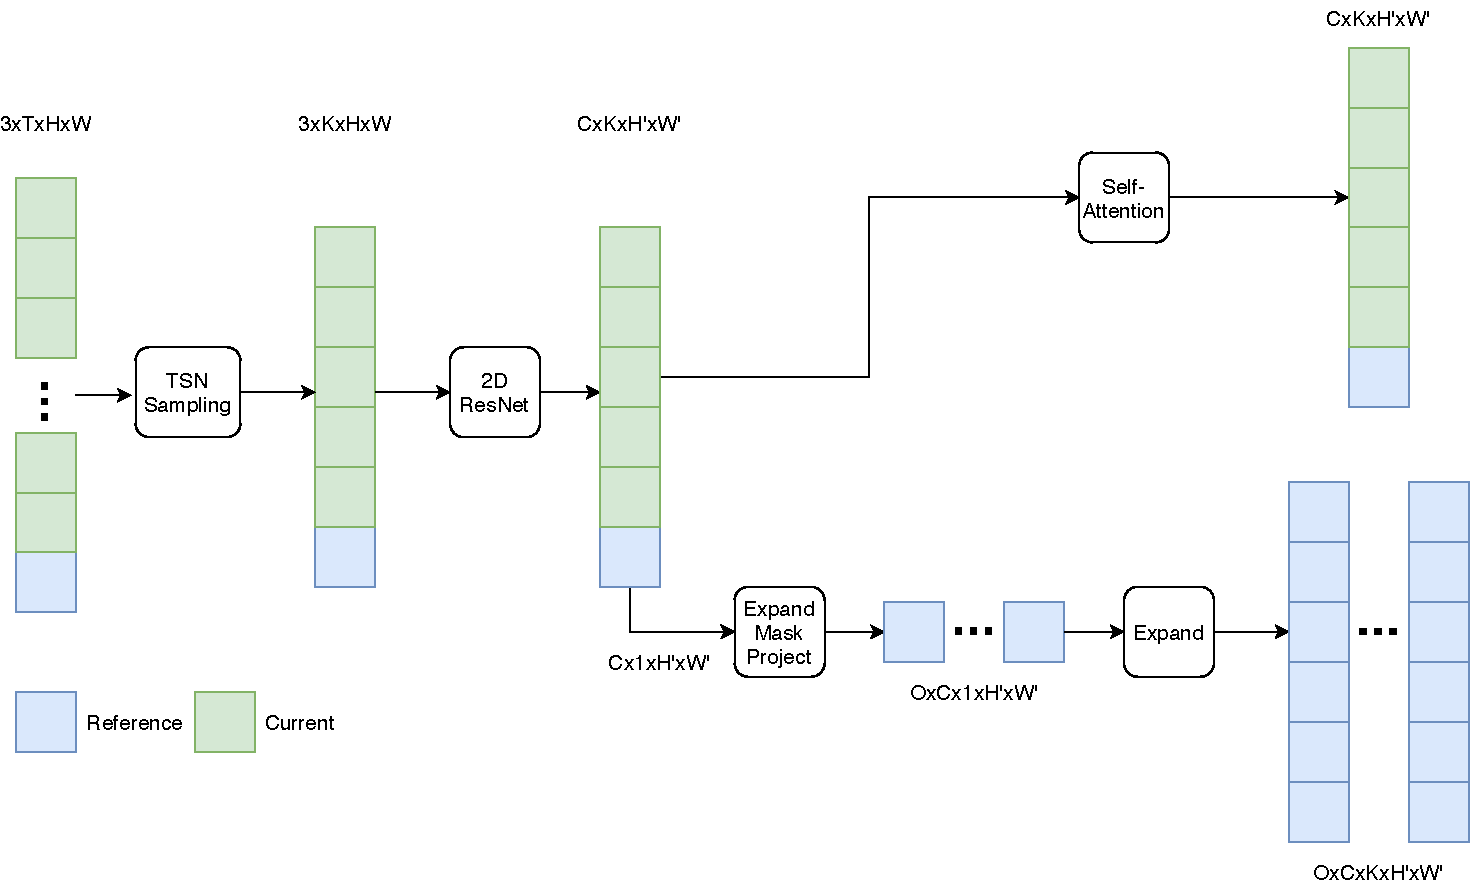
\includegraphics[width=1.0\textwidth]{Figures/aina_encoder.pdf}
\caption{SST encoder architecture.
         The input to the SST encoder is a
         video~$\in\real{}^{3\times T \times H\times W}$, where~$T$ is the
         total number of video frames.
         From left to right, the video is first subsampled (using TSN
         sampling~\citep{wang2016temporal} during training) to a fixed number of
         frames~$K$, which are processed independently by a 2D
         ResNet~\citep{he2016deep} to produce a feature tensor~$\in
         \real{}^{C\times K \times H'\times W'}$.
         The encoder then splits into two representation streams.
         The top stream encodes generic video features, and incorporates
         temporal context using a self-attention layer.
         The bottom stream encodes object-discriminative features by applying
         the Expand-Mask-Project operator to the reference features, and
         repeating the resultant feature tensor~$K$ times.
         Both streams are input to the SST decoder, described in
         Figure~\ref{fig:ainadecoder}.
         Blue indicates reference features and green indicates non-reference
         video features (best viewed in colour).}
\label{fig:ainaencoder}
\end{figure*}

The Expand-Mask-Project layer (Figure~\ref{fig:expandmaskproject}) relays to
the decoder information about whether each pixel in the feature map belongs to
an object by projecting object foreground and background to different affine
subspaces described by the parameters of affine
transformations~$T_{foreground}$ and~$T_{background}$.

To separately project object foreground and background features we use each
object's downsampled mask and inverse mask (i.e.,~$1 - M$ for binary object
mask~$M$) to extract object foreground and background features.
Foreground and background affine transformations~$T_{foreground}$
and~$T_{background}$ then project their respective extracted features to
foreground and background affine subspaces.
An elementwise addition operation then combines the projected object foreground
and background features, producing a single~$O\times C\times H'\times W'$
reference feature map, where~$O$ is the number of objects and~$C$ the number of
channels, that contains information about which pixels of the feature map
belong to which object.

Finally, the SST encoder's object-discriminative stream repeats the projected
object foreground and background features by the number of sampled frames~$K$
times along a new axis to produce an~$O\times C\times K\times H'\times W'$
output to feed into the SST decoder.

We briefly justify our choice to repeat the projected reference features across
the video.
The SST decoder gradually updates the object-discriminative features to produce
the video object segmentation.
When the SST encoder passes its object-discriminative features to the decoder,
the encoder has not yet incorporated temporal context.
Therefore, repeating the projected reference features across the video is the
encoder's best initialization for object location throughout the video based
only on the prior knowledge given in the reference frame.

\begin{figure}
\centering
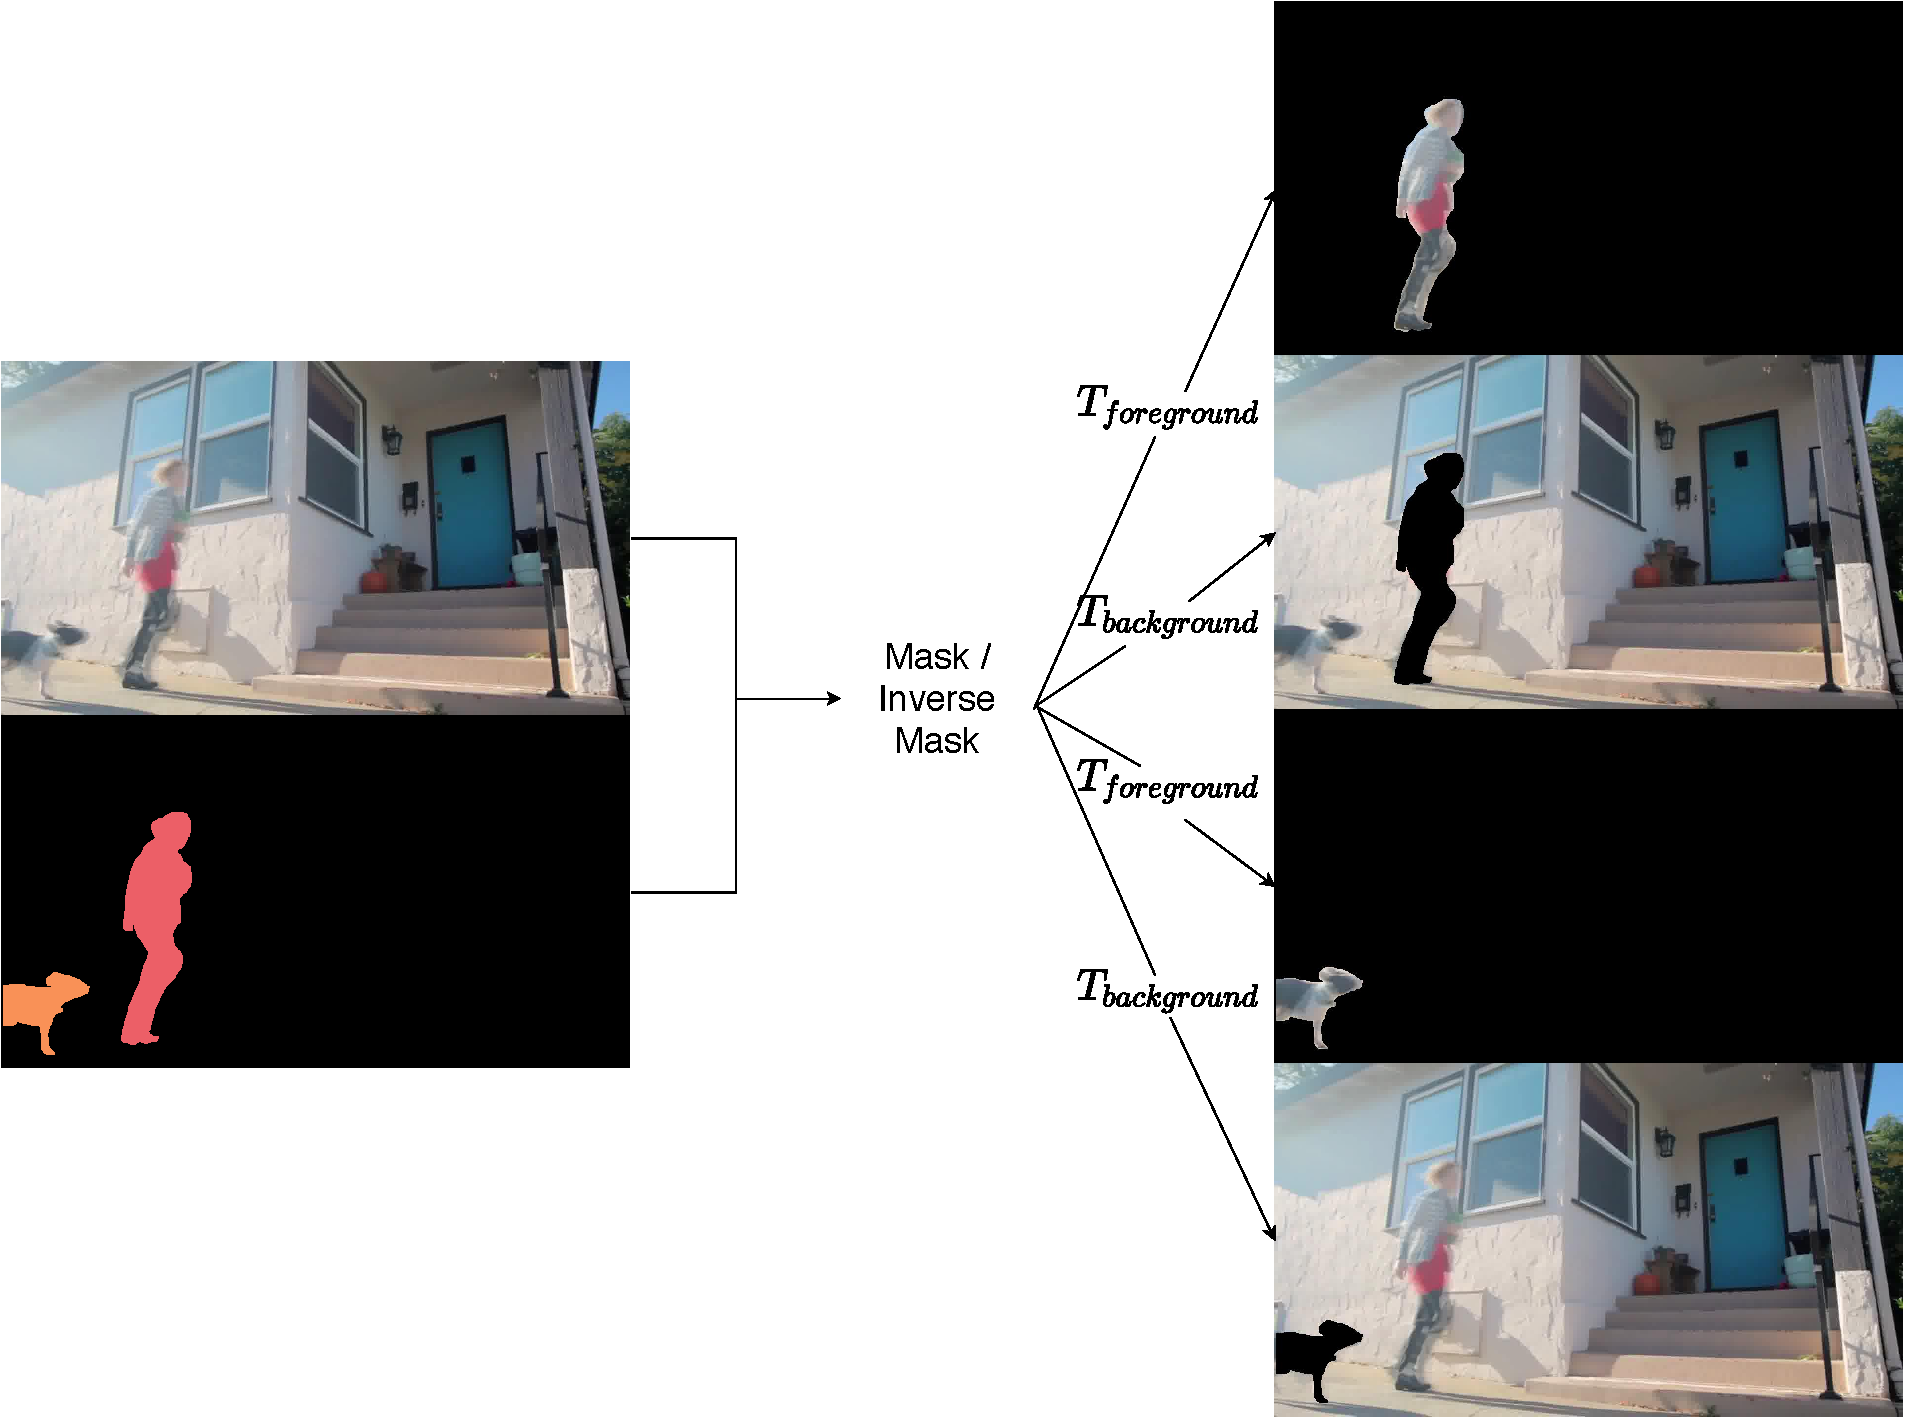
\includegraphics[width=0.9\textwidth]{Figures/expand-mask-project.pdf}
\caption{Expand-Mask-Project operator.
         We use an RGB image to visualize feature maps for clarity.
         The actual Expand-Mask-Project operator uses downsampled object masks
         and reference features processed by a 2D ResNet~\citep{he2016deep} of
         stride~\num{8}.
         % TODO(brendan): replace with feature visualization from actual model
         % (e.g., SSS visualization).
         The Expand-Mask-Project operator has three steps: \textbf{Expand},
         \textbf{Mask}, and~\textbf{Project}.
         In the~\textbf{Expand} step, we repeat the~$C\times H'\times W'$
         reference features along a new object axis to get
         an~$O\times C\times H'\times W'$ tensor, where~$O$ is the number of
         objects to segment.
         We then use each object~$o$'s foreground mask~$M_o$ and corresponding
         background mask~$1 - M_o$ in the~\textbf{Mask} step to create two
         copies of the original feature map for each object: one with only that
         object (and the background zero'ed out), and the other with only the
         background (i.e., everything besides the object, and the object
         zero'ed out).
         Finally, in the~\textbf{Project} step, we use affine
         transformations~$T_{foreground}$ and~$T_{background}$ to separately
         project each object's foreground and background to the affine
         subspaces designating foreground and background features,
         respectively.}
\label{fig:expandmaskproject}
\end{figure}

% TODO(brendan): to align this better with NLP Transformer, the
% Expand-Mask-Project operator could be moved into the decoder.
The SST encoder produces two outputs passed to the SST decoder: a generic video
feature representation~$\vidfeat{}\in\real{}^{C\times K \times H'\times W'}$,
and an initial object-discriminative video feature
representation~$\objfeat{}\in\real{}^{O\times C\times K \times H'\times W'}$.

The SST decoder, shown in Figure~\ref{fig:ainadecoder}, is a sequence of
cross-attention layers that match object-discriminative and generic video
features to warp the video object representation prior to the object's features
throughout the video.
The final layer of the SST decoder is a scoring convolution and sigmoid (at
training time) or argmax (at test time) layer that produces the video object
segmentation probability or segmentation
masks~$\outputvar{} \in \real{}^{K\times H\times W}$ from the final
object-discriminative representation.
In the case of multiple objects we have probability scoremaps
in~$\real{}^{O\times 2\times K\times H\times W}$, i.e., foreground-background
probabilities for each object for each pixel in the video, which we want to
reduce to a tensor in~$\real{}^{K\times H\times W}$ of object integer labels.
We use the ``na\"ive'' inference protocol~\citep{oh2018fast} and take, for each
pixel, the argmax over all object probabilities including the background
probability, computed as the maximum background probability over all objects.

As we elaborate on in Section~\ref{sec:sparse-attn}, each cross-attention layer
takes query~$\querytensor{}$, key~$\keytensor{}$, and value~$\valuetensor{}$
tensors as input and returns a weighted sum of~$\valuetensor{}$, where the
weight of each value at an index in~$\valuetensor{}$ increases with the dot
product of the query and key at the same index.
In the SST decoder, the role of query is played by the video representation,
while the object-discriminative representation plays the role of both key and
value, such that the function signature of each attention layer
is~$\mathtt{Attention}\big(\querytensor{} = \vidfeat{}, \keytensor{} = \objfeat{}, \valuetensor{} = \objfeat{}\big)$.
Note that in object-discriminative features~$\objfeat{}$ foreground and
background have been projected to separate affine subspaces, and we can use the
projection weights in attention to perform a lookup in either of those
subspaces to match against our video features.

From the perspective of attention as mapping a query and key-value pair, at
each step we use feature vectors from our evolving object-discriminative
representation to query the video key-value pair.
We update our previous estimate of the video object-discriminative features
with the resulting linear combination of video features from this lookup.
Intuitively, we use our prior knowledge about reference features to perform a
search in the video feature tensor to find features similar to our object.
In subsequent steps we reuse the results of previous queries to perform a
cascade of new searches for the object using our updated object feature
estimate.

% TODO(brendan): use vidfeat and objfeat notation should be in the figure.
\begin{figure*}
\centering
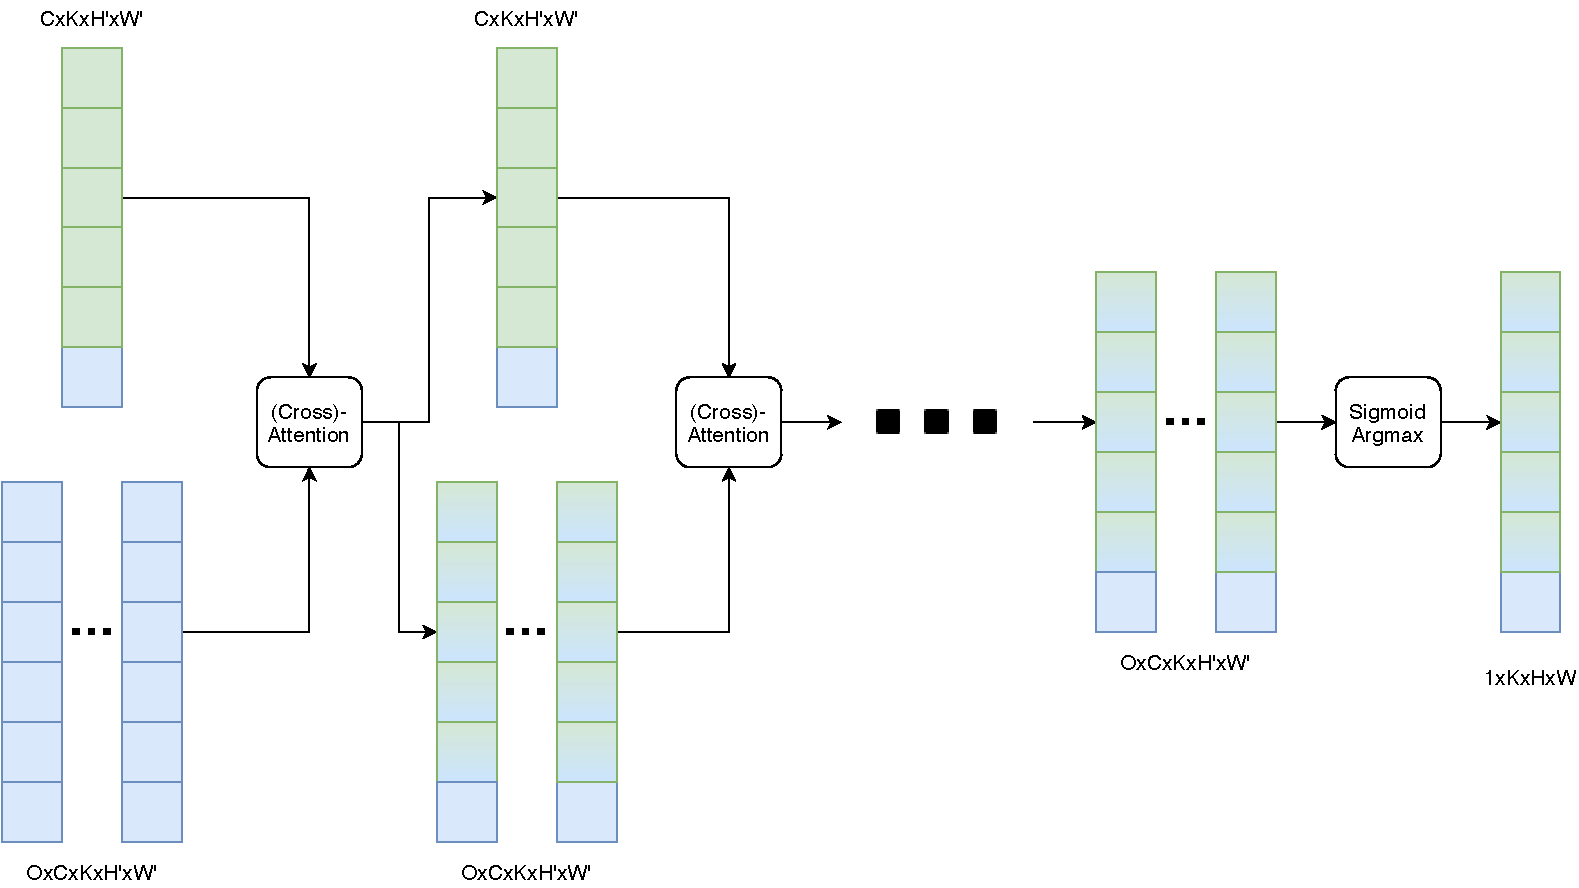
\includegraphics[width=1.0\textwidth]{Figures/aina_decoder.pdf}
\caption{SST decoder architecture.
         Decoder inputs are a generic video representation
         tensor~$\vidfeat{}\in\real{}^{C\times K \times H'\times W'}$ (top
         left, blue and green), along with object-discriminative reference
         features~$\objfeat{}\in\real{}^{O\times C\times K \times H'\times W'}$
         (bottom left, blue), where~$O$, $C$, $K$ and~$H'\times W'$ denote the
         number of objects, feature channels, subsampled video frames, and
         video spatial dimensions, respectively.
         The SST decoder is a series of cross-attention layers that warp
         reference features~$\objfeat{}$ to follow objects' movements in the
         video by matching with video features~$\vidfeat{}$.
         We use colour gradients to show that object representations after the
         decoder input are a mixture of object-specific (blue) and generic
         video (green) features, therefore this figure is best viewed in
         colour.}
\label{fig:ainadecoder}
\end{figure*}


\subsection{Sparse Attention}
\label{sec:sparse-attn}

Attention is a dense operator that allows each element of a tensor to interact
with all other elements at each attention layer.
Attention is desirable in VOS because it can capture long-range dependencies
without recurrence, and because attention can be viewed intuitively as a
cross-correlation operator that uses CNN features for
correspondence~\citep{long2014correspondence}, similar to prior work that used
matching layers for optical flow~\citep{dosovitskiy2015flownet}.

Formally, we follow~\citet{vaswani2017attention} in defining attention as

\begin{equation}
\mathtt{Attention}\big(\querytensor{}, \keytensor{}, \valuetensor{}\big) = \softmax{}\big(\querytensor{}\keytensor{}^\top\big)\valuetensor{},
\label{eqn:attndefn}
\end{equation}

\noindent where query~$\querytensor{}$, key~$\keytensor{}$, and value~$\valuetensor{}$
are all matrices in~$\real{}^{S\times C}$ for flattened spatial dimensions~$S =
THW$.
As we alluded to in Section~\ref{sec:architecture}, we use object
discriminative features~$\objfeat{}$ as query, and generic video
features~$\vidfeat{}$ as both key and value.
Intuitively we use object-discriminative features initialized by the reference
features to do a lookup in the video features in order to update our video
object features estimate.

We adapted for VOS characteristic components of the Transformer architecture as
described by \citet{vaswani2017attention}, including multi-head
attention and positional encodings.
We compare the performance of different positional encoding schemes applied to
VOS in Section~\ref{sec:yvosablation}.
We did not normalize the softmax argument in Equation~\ref{eqn:attndefn} by the
inverse square root of channels, as we found this scaling factor hurt
performance.
The difference in impact of scaling factor between our VOS attention and
Vaswani et al.'s NLP attention could be due to our attention operator having a
comparatively low number of channels.

A computational barrier prevents na\"ively using Equation~\ref{eqn:attndefn} to
perform our desired lookup of video features~$\vidfeat{}$ using
object-discriminative features~$\objfeat{}$.
The attention operation given in Equation~\ref{eqn:attndefn} is~$O({(THW)}^2
C)$, which poses a problem for video object segmentation since for dense
prediction tasks such as segmentation, model performance tends to improve with
greater input resolution~\citep{zhao2017icnet}.
As an illustration of the infeasibility of using na\"ive attention for VOS,
consider that a single layer of attention on a~\num{16} frame video with
a~$64\times 64$ feature map with~\num{32} channels would cost more
than~\num{137} billion FLOPs, far more than the most computationally expensive
CNNs in the literature at the time of writing~\citep{tan2019efficientnet}.

We used two different sparse attention methods to make our attention operator
computationally tractable at our desired framerate and resolution.


\subsubsection{Grid Attention}

We adapted our first sparse attention operator from Huang et al., who also
noted the computational complexity issue when applying attention for semantic
segmentation~\citep{huang2018ccnet}, although in VOS the issue is exasperated
further by the addition of the time dimension.
We refer to this operator as grid attention since we have generalized it from
two to three dimensions, where the moniker criss-cross attention is no longer
fitting.

At each layer of grid attention, each pixel of the video feature activation
aggregates information from other pixels along its~$X$,~$Y$, and~$T$ axes
independently.
Each pixel interacts once with every other pixel in the video feature
activation tensor that shares at least two of its~$X$,~$Y$, and~$T$
coordinates.
Formally, for query~$\querytensor{}$, key~$\keytensor{}$, and
value~$\valuetensor{}$ tensors all in~$\real{}^{C\times T\times H\times W}$, we
define our~$\mathtt{GridAttention}$ operator as

\begin{equation}
\mathtt{GridAttention}{\big(\querytensor{}, \keytensor{}, \valuetensor{})} = \Phi\big(\Omega\big(\querytensor{}, \keytensor{}\big), \valuetensor{}\big),
\label{eqn:gridattndefn}
\end{equation}

\noindent where~$\Phi$ and~$\Omega$ are the 3D generalizations of
the~\textbf{aggregation} and~\textbf{affinity} operations defined by
\citet{huang2018ccnet}.

Concretely, we define affinity operator~$\Omega$ as

% TODO(brendan): introduce superscript notation instead of Psi
% function, since superscript is more compact.
\begin{equation}
        {\Omega\big(\querytensor{}, \keytensor{}\big)}_\pixel{} = \softmax{}\big(\querytensor{}_\pixel{} {\Psi\big(\keytensor{}, \pixel{}\big)}^\top\big)
\label{eqn:gridattndefn}
\end{equation}

\noindent where~$\Psi : \real{}^{S\times C} \times \real{}^3 \rightarrow \real{}^{(T + H + W - 2)\times C}$
returns all pixels along the horizontal, vertical, or temporal axes incident to
location~$\pixel{} \equiv (x, y, t)$.
$\Omega(\querytensor{}, \keytensor{})$ is then a matrix
in~$\real{}^{S\times (T + H + W - 2)}$ where each row contains, for a pixel in
the video feature tensor, weights of a weighted average over all pixels along
its temporal, vertical, and horizontal axes.

Aggregation operator~$\Phi$ computes for each pixel~$\pixel{}$ in the video
feature tensor a weighted average over pixels along the temporal, vertical, and
horizontal axes incident to~$\pixel{}$.
Concretely, we
define~$\Phi : \real{}^{S\times (T + H + W - 2)} \times \real{}^{S\times C} \rightarrow \real{}^{S\times C}$
as

\begin{equation}
        {\Phi\big(A, \valuetensor{}\big)}_\pixel{} =  {A_\pixel{}}^\top \Psi\big(\valuetensor{}, \pixel{}\big).
\end{equation}

Note that we implemented our grid attention operator in place, so there is no
overhead from indexing tensors by~$\pixel{}$.

\begin{figure}
\centering
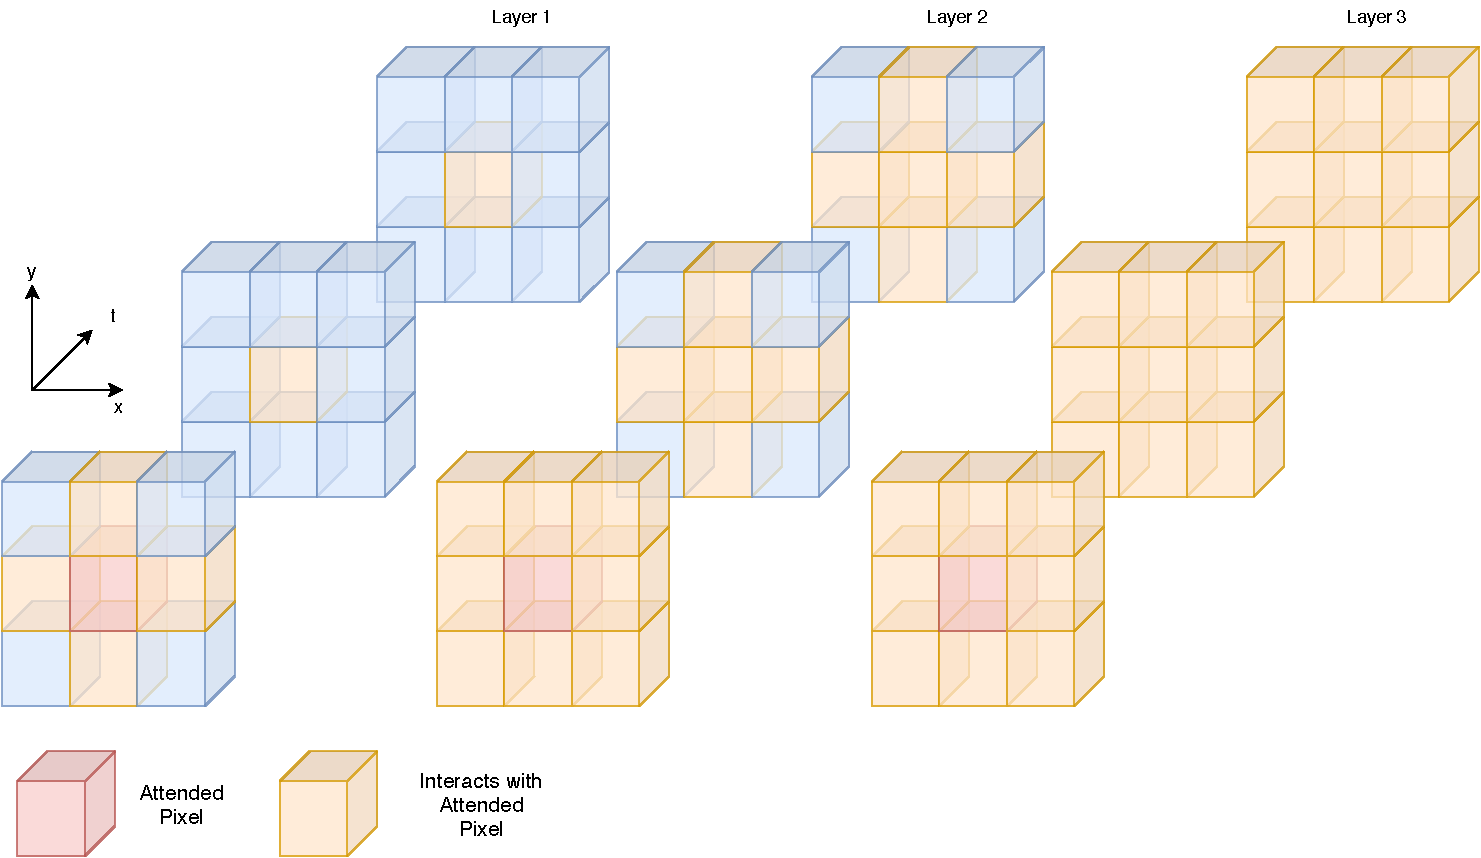
\includegraphics[width=0.9\textwidth]{Figures/gridattention.pdf}
\caption{Interaction propagation from a given pixel via grid attention.}
\label{fig:ainadecoder}
\end{figure}

In Figure~\ref{fig:ainadecoder} we illustrate how grid attention propagates
interactions from a single attended pixel to all other pixels in three
sequential layers.
The first grid attention layer propagates information to other pixels in the
same frame vertically and horizontally, and to pixels at the same spatial
location in all other frames.
The second layer propagates interactions to the entire current frame, and
vertical and horizontal axes in other frames.
Finally, the third layer propagates information to all pixels in the video
feature tensor.

% TODO(brendan): the presentation may make more sense if we use the
% reference-fg/bg features as key-value, and the video features as query.
% Then we can use the example of R = fg/bg mask to warp the mask through
% transitive correlation of video features with the reference.
To demonstrate mathematically information propagation in grid attention we
consider, for sake of clarity, a function~$\tilde{\Omega}$ that is~$\Omega$
without the softmax in Equation~\ref{eqn:gridattndefn}.
Further assume that our query is our video feature tensor, and our key and
value are both our object feature tensor,
i.e.,~$\querytensor{} = \vidfeat{}$,~$\keytensor{} = \objfeat{}$,
and~$\valuetensor{} = \objfeat{}$.
The first layer outputs, for each pixel~$\pixel{} \equiv (x, y, t)$,

\begin{equation}
\begin{split}
        \Phi{\big({\tilde{\Omega}\big(\vidfeat{}, \objfeat{}\big)}, \objfeat{}\big)}_{xyt} =
        & \sum_{i = 1}^W \big(\vidfeat{}_{xyt}^\top\objfeat{}_{iyt}\big)\objfeat{}_{iyt} + \\
        & \sum_{\substack{j = 1 \\ j \neq y}}^H \big(\vidfeat{}_{xyt}^\top \objfeat{}_{xjt}\big)\objfeat{}_{xjt} + \\
        & \sum_{\substack{k = 1 \\ k \neq t}}^T \big(\vidfeat{}_{xyt}^\top \objfeat{}_{xyk}\big)\objfeat{}_{xyk}
\end{split}
\end{equation}

We can show that composing one application of~$\Phi$ and~$\tilde{\Omega}$ with
two applications of self-attention on~$\vidfeat{}$, which we denote for brevity
as~$\Phi^3_{\tilde{\Omega}}$, produces

\begin{equation}
\begin{split}
        {\Phi^3_{\tilde{\Omega}}\big(\vidfeat{}, \objfeat{}\big)}_{xyt} =
                \sum_{i = 1}^W \sum_{j = 1}^H \sum_{k = 1}^T
                & \big(\vidfeat{}_{xyt}^\top\vidfeat{}_{iyt}\big) \\
                & \big(\vidfeat{}_{iyt}^\top \vidfeat{}_{ijt}\big) \\
                & \big(\vidfeat{}_{ijt}^\top \objfeat{}_{ijk}\big)\objfeat{}_{ijk} + \cdots,
\end{split}
\label{eqn:gridattnrouting}
\end{equation}

\noindent where~$\cdots$ represents other similar third order terms.
We show in Equation~\ref{eqn:gridattnrouting} that grid attention propagates
information along ``routes'' through the video feature tensor: for a pixel at
position~$(x, y, t)$ to interact with another pixel at an arbitrary
position~$(i, j, k)$, interactions must propagate along a ``route''  through
the video feature tensor of pairs of similar pixels.
Just as we might give travel directions through a city grid such as ``first
walk ten blocks North, then walk three blocks East'', grid attention
interactions must propagate a fixed number of pixels in the~$X$,~$Y$ and~$T$
directions, in some order, before connecting the interaction source pixel with
its target pixel.

Consider what happens if we replace the value~$\objfeat{}_{ijk}$ returned by
the inner cross-attention in Equation~\ref{eqn:gridattnrouting} with a
foreground mask value~$m_{ijk}$.
We see that the output routes reference mask values~$m_{ijk}$ over paths of
feature vectors in the video tensor~$\vidfeat{}$ that transitively correspond
to reference features~$\objfeat{}_{ijk}$.

By replacing dense attention with grid attention we reduced the computational
complexity of video attention from~$O(C{(THW)}^2)$ to~$O(C(T + H + W)THW)$,
achieving our goal of making attention tractable for video.

% TODO(brendan): unify language and notation with grid attention
%
% Path of locations


\subsubsection{Strided Attention}

We also investigated strided attention as an alternative sparse attention
method in addition to grid attention.
Drawing inspiration from \citet{child2019sparsetransformer}, we
propagate information by following paths of locations through sparse
connectivity patterns in our video feature tensor.
We define a connectivity
pattern~$I = \{I_{\pixel{}_0}, \dots, I_{\pixel{}_S}\}$
where~$I_\pixel{}$ is a set of coordinates~$(i, j, k)$ that index a 3D tensor.
Each layer of strided attention then returns, for each pixel~$\pixel{}$,

\begin{equation}
\mathtt{StridedAttn}{\big(\querytensor{}, \keytensor{}, \valuetensor{})}_\pixel{} = \softmax{}\big(\querytensor{}_\pixel{} \keytensor{}^\top_{I_\pixel{}}\big)\keytensor{}_{I_\pixel{}}.
\label{eqn:stridedattndefn}
\end{equation}

We define~$I_\pixel{}$ as a generalization of Child et al.'s strided attention
from 1D to 3D\@.
Our strided attention uses two different connectivity patterns~$I^1_\pixel{}$
and~$I^2_\pixel{}$ corresponding to separate, sequential heads of multihead
attention.
The first connectivity pattern~$I^1_\pixel{}$ routes to all pixels in a cube of
side-length~$h$ from~$\pixel{}$,
i.e.,~$I^1_\pixel{} = (\pixel{} + (l_x, l_y, l_z) \,:\, l_x, l_y, l_z < h)$.
The subsequent connectivity pattern~$I^1_\pixel{}$ routes to all pixels in the
video tensor that can reach~$\pixel{}$ by taking steps of size~$h$ along each
axis,
i.e.,~$I^2_\pixel{} = (\pixel{} + (l_x, l_y, l_z) \,:\, l_x, l_y, l_z \mod h = 0)$.
We choose~$h\approx \sqrt{H}$ to reduce the computational complexity by a
square root to~$O(C{(THW)}^{3/2})$ from~$O(C{(THW)}^2)$.

The relative efficiency of grid and sparse attention depends on the size
of~$T$, since we assume that~$H$ and~$W$ are comparably large and both larger
than~$T$.
During training when we subsample video sequences, sparse attention costs
about~\num{1.3} to~\num{1.4} times as many operations as grid attention, given
our training configuration where~$H, W \in \{64, 128\}$, and~$T\approx 8$.
% TODO(brendan): actual training sampling strategy for strided attention, after
% experimenting
% TODO(brendan): do Child et al. even address cross-attention?


\subsection{Appearance Model}

% Long et al.\ showed that ConvNets learn correspondence, and furthermore ConvNet
% features can align intraclass instances~\citep{long2014correspondence}.
% By using attention for VOS we leverage this correspondence property of ConvNet
% features in order to do pixelwise tracking.  However, to adapt attention to VOS
% we must extract representations that distinguish one object from another,
% whereas Long et al.\ showed that intraclass ConvNet features match so well that
% they are effective for intraclass alignment~\citep{long2014correspondence}.
% Therefore we introduce ``Attention in Attention'', an operator responsible for
% adaptively adjusting object representations to become discriminative features
% even in the presence of multiple instances of the same class.

% Our ``Attention in Attention'' (AIA) operator adaptively updates appearance
% models of each object through inter-object attention.
Johnander et al.\ showed that appearance models are effective for VOS,
particularly in generalizing to classes not seen in the training
set~\citep{johnander2019agenerative}.  Hence, following Johnander et al., we
define object appearance models as

\begin{subequations}
\begin{align}
        \objmean{} &= \frac{\sum_\pixel{}\alpha_{\pixel{}, o} x_\pixel{}}{\sum_\pixel{}\alpha_{\pixel{}, o}} \\
        \objcov{} &= \frac{\sum_\pixel{}\alpha_{\pixel{}, o} \mathrm{diag}\{{(x_p - \objmean{})}^2 + r_k\}}{\sum_\pixel{}\alpha_{\pixel{}, o}}
\end{align}
\label{eqn:appearancemodel}
\end{subequations}

\noindent where~$o$ indexes objects in the video,~$\pixel{}$ indexes pixels in the
video,~$\alpha_{\pixel{}, o} \in \{0, 1\}$ indicates whether a given
pixel~$\pixel{}$ in the reference frame belongs to object~$o$,
and~$r_k$ are model parameters.

Since~$\alpha_{\pixel{}, o}$ takes discrete values of unity inside an object,
and zero outside, in our current definition we still form object appearance
models~$(\objmean{}, \objcov{})$ independently of other objects in a video.
We hypothesize that future work on a learned component that incorporates
explicit knowledge about visual context, including both other objects and
background, into an object's appearance model would improve the ability to
extract object representations that are discriminative.

The log probability of a pixel's feature vector being generated by a given
object's appearance model forms an additional feature, which is concatenated to
the input to the self-attention block in the SST encoder.

% We use AIA to adaptively incorporate visual context into the appearance model
% defined in Equation~\ref{eqn:appearancemodel}.
% We define AIA as a dense attention operation between the appearance models of
% all objects in a video, as well as the background.
% Concretely, let~$U \in \real{}^{(O + 1)\times C}$ be the matrix of object
% appearance model means~$\objmean{}$, including the background.
% We compute an attention matrix~$A\in \real^{(O + 1)\times (O + 1)}$ as

% \begin{equation}
% A = \softmax{\big(UW_q {(UW_k)}^\top\big)}.
% \end{equation}

% Then we update each object~$o$'s appearance model~$\objmean{}$ to become a
% visual-context-aware appearance model~$\objctx{}$, defined as

% \begin{equation}
%         \objctx{} = \objmean{} + {(AUW_v)}_k.
% \end{equation}

% where~${(AUW_v)}_k$ is the~$o$th row of attention over objects, which provides
% a weighting over object means~$U$ projected by learned weights~$W_v$.

% AIA gives our appearance models the ability to incorporate visual context from
% other objects and background.
% For example, if two objects~$o$ and~$l$ have appearance models with a
% difference vector~$\bm{\mu}_k - \bm{\mu}_l \equiv \Delta$, AIA can update both
% objects to be more distinguishable so
% that~$\tilde{\bm{\mu}}_k - \tilde{\bm{\mu}}_l = \alpha\Delta$ for~$\alpha > 1$.
% In Section~\ref{sec:experiments} we demonstrate improvement from adding the AIA
% operator.


\section{Experiments and Results}
\label{sec:experiments}

We present benchmark experiment results against state-of-the-art (SOTA) methods
on the DAVIS 2016~\citep{perazzi2016abenchmark}, DAVIS
2017~\citep{ponttuset2017davis}, and YouTube-VOS~\citep{xu2018youtubevos}
datasets.
% We further analyze the effect of different sparse attention operators,
% positional encodings, and AIA operator variations through ablation studies
% using YouTube-VOS\@.
We further analyze the effect of different sparse attention operators and
positional encodings through ablation studies using YouTube-VOS\@.


\subsection{YVOS}
% YVOS comparison to SOTA

\begin{table}
\caption{Comparison with SOTA methods on YouTube-VOS~\citep{xu2018youtubevos}.
         We compute region similarity~\J{} over seen and unseen
         categories, then average those scores with contour
         accuracy~\F{} seen and unseen to get overall
         score~\G{}.
         We compute region similarity and contour accuracy as
         in~\citet{perazzi2016abenchmark}.
         We distinguish methods by those that use online finetuning (O-Ft), and
         those that do not.}
\centering
\begin{tabular}{@{}lcrrr@{}}
\toprule
Method & O-Ft & \begin{tabular}{@{}r@{}}\G{} overall \\ (\%)\end{tabular} & \begin{tabular}{@{}r@{}}\J{} seen \\ (\%)\end{tabular} & \begin{tabular}{@{}r@{}}\J{} unseen \\ (\%)\end{tabular} \\
\midrule
S2S~\citep{xu2018youtube} & \yesmark & 64.4 & 71.0 & 55.5 \\
OSVOS~\citep{caelles2017one} & \yesmark & 58.8 & 59.8 & 54.2 \\
OnAVOS~\citep{voigtlaender2017online} & \yesmark & 55.2 & 60.1 & 46.6 \\
MSK~\citep{khoreva2017learning} & \yesmark & 53.1 & 59.9 & 45.0 \\
\addlinespace[1mm]
OSMN~\citep{yang2018efficient} & \nomark & 51.2 & 60.0 & 40.6 \\
S2S~\citep{xu2018youtube} & \nomark & 57.6 & 66.7 & 48.2 \\
RGMP~\citep{oh2018fast} & \nomark & 53.8 & 59.5 & 45.2 \\
A-GAME~\citep{johnander2019agenerative} & \nomark & 66.0 & 66.9 & \textbf{61.2} \\
\textbf{SST (Grid)} & \nomark & 66.5 & 67.8 & 60.2 \\
\textbf{SST (Strided)} & \nomark & \textbf{68.1} & \textbf{69.9} & 60.8\\
\bottomrule
\end{tabular}
\label{tab:sota-yvos}
\end{table}

YouTube-VOS~\citep{xu2018youtubevos} is a large scale VOS dataset comprised
of~\num{4453} YouTube video clips spanning~\num{94} object categories.
YouTube-VOS includes an official validation set of~\num{474} videos with
heldout labels, which can be evaluated only through an evaluation server.
The YouTube-VOS validation set contains~\num{26} object categories that are
unique to the validation set, used to test the generalization capability of VOS
models to object classes unseen in the training set.
The convention is to compute region similarity~\J{} and contour accuracy~\F{}
as defined by \citet{perazzi2016abenchmark}.
As a single metric for comparing results, it is also customary to compute
overall score~\G{} as the average of four values comprising region similarity
and contour accuracy scores for seen and unseen classes.

In Table~\ref{tab:sota-yvos} we present our model's results on YouTube-VOS
alongside previous SOTA results.
Our model (SST) performs favourably against all previous methods in overall
score~\G{}, even methods that use online finetuning (denoted by O-Ft).

Note that our unique method performs competitively against recurrent methods
that have undergone multiple research and development cycles where one method
builds on the foundation of another, for
example~\citet{johnander2019agenerative} extends~\citet{oh2018fast}, which in
turn extends~\citet{khoreva2017learning}.


\subsection{DAVIS}
% DAVIS comparison to SOTA

% TODO(brendan): runtime comparison?
\begin{table}
\caption{Comparison with SOTA methods on DAVIS2017~\citep{ponttuset2017davis}.}
\centering
\begin{tabular}{lcrrr}
\toprule
Method & O-Ft & \begin{tabular}{@{}r@{}}\JandF{} mean \\ (\%)\end{tabular} & \begin{tabular}{@{}r@{}}\J{} \\ (\%)\end{tabular} & \begin{tabular}{@{}r@{}}\F{} \\ (\%)\end{tabular} \\
\midrule
CINM~\citep{bao2018cnn} & \yesmark & 70.6 & 67.2 & 74.0 \\
OSVOS-S~\citep{maninis2018video} & \yesmark & 68.0 & 64.7 & 71.3 \\
OnAVOS~\citep{voigtlaender2017online} & \yesmark & 65.4 & 61.6 & 69.1 \\
OSVOS~\citep{caelles2017one} & \yesmark & 60.3 & 56.6 & 63.9 \\
\addlinespace[1mm]
DyeNet~\citep{li2018video} & \nomark & 69.1 & 67.3 & 71.0 \\
RGMP~\citep{oh2018fast} & \nomark & 66.7 & 64.8 & 68.6 \\
VM~\citep{hu2018videomatch} & \nomark & - & 56.5 & - \\
FAVOS~\citep{cheng2018fast} & \nomark & 58.2 & 54.6 & 61.8 \\
OSMN~\citep{yang2018efficient} & \nomark & 54.8 & 52.5 & 57.1 \\
A-GAME~\citep{johnander2019agenerative} & \nomark & 70.0 & 67.2 & 72.7 \\
\textbf{SST (Strided)} & \nomark & \davisvalG & 50.5 & 55.9 \\
\bottomrule
\end{tabular}
\label{tab:sota-davis}
\end{table}

DAVIS2017 is the latest dataset in the DAVIS initiative to promote VOS
research.
DAVIS2017 comprises 150 sequences, which include 376 separately annotated
objects~\citep{ponttuset2017davis}.

We additionally evaluate our method on DAVIS2017~\citep{ponttuset2017davis}, and
compare our results with SOTA in Table~\ref{tab:sota-davis}.
We report our DAVIS results following the traditionally used region
similarity~\J{} and contour accuracy~\F{} metrics as well as their
mean~\JandF{}.
% Our DAVIS2017 evaluation provides additional experimental evidence that SST
% method performs favourably compared with existing SOTA methods, since SST
% achieves a mean~\JandF{} score of~$\davisvalG$, whereas previous SOTA scored
% a~\JandF{} of~\num{70.6}.
According to our DAVIS2017 evaluation, SST performs relatively poorly
compared to prior work, since SST achieves a mean~\JandF{} score
of~$\davisvalG$, whereas previous SOTA scored a~\JandF{} of~\num{70.6}.
We believe that our method's performance on the DAVIS2017 validation set is
reflective of a weakness of our current formulation.
The DAVIS2017 validation set is made up of only~\num{30} sequences, and since
the DAVIS2017 evaluation is done per object, sequences with many objects are
weighed far heavier in the evaluation.
For example, a single sequence with a group of people dancing accounts for more
than~\num{10}\% of the final score.

We hypothesize that our method performs poorly on exactly the sequences that
DAVIS2017 weighs heavily in evaluation, where there are many objects of the
same class that need to be tracked in a video.
We observe that in these cases our method performs well in the initial frames,
and then our method's performance deteriorates rapidly.
SST's most common failure mode is confusing multiple objects of the same class
in medium and long temporal sequence lengths.

Long et al.\ showed that ConvNets learn correspondence, and furthermore ConvNet
features can align intraclass instances~\citep{long2014correspondence}.
By using attention for VOS we leverage this correspondence property of ConvNet
features in order to do pixelwise tracking.
However, to adapt attention to VOS we must extract representations that
distinguish one object from another, whereas Long et al.\ showed that
intraclass ConvNet features match so well that they are effective for
intraclass alignment.
We believe that the inductive bias of recurrent methods gives a temporal cue to
the VOS model to favour matching features that are spatially nearby, since
recurrent methods always propagate information from the previous frame.
Since our method currently lacks this inductive bias, our model is unable to
separate objects of the same class beyond the initial frames close to the
reference frame.
In future work we propose to inject this same ``spatial locality'' inductive
bias into SST by updating our object-discriminative and reference features
gradually with the predictions from earlier layers, instead of simply
initializing object-discriminative and reference features with the reference
frame.

We evaluate only on DAVIS2017 and not DAVIS2016~\citep{perazzi2016abenchmark}
because DAVIS2017 is strictly a more challenging superset of DAVIS2016.
Furthermore DAVIS2016 contains only single object annotations and therefore we
could make only limited evaluation of SST's ability to handle multi-object
context using DAVIS2016.
In general we consider YouTube-VOS the currently most superior benchmark for
comparing VOS algorithms due to its large size, variety, evaluation on a
heldout set using an evaluation server, as well as its unseen classes, which
are useful for evaluating generalization.


% TODO(brendan): MOTS comparison to SOTA (time permitting)


\subsection{Ablation Studies}
\label{sec:yvosablation}
% YVOS ablation studies

% \begin{table}
% \caption{Performance decay evaluation on DAVIS2017~\citep{ponttuset2017davis}.}
% \centering
% \begin{tabular}{lccr}
% \toprule
% Method & O-Ft & Recurrent & $\mathcal{D}$ \\
% \midrule
% RGMP~\citep{oh2018fast} & \nomark & \yesmark & \\
% \textbf{SST} & \nomark & \nomark & 0.21 \\
% \bottomrule
% \end{tabular}
% \label{tab:decay}
% \end{table}

We were motivated to use attention-based models for VOS due to spatiotemporal
attention's ability to incorporate temporal context without incurring a decay
in performance due to accumulating errors as is inherent to reccurent and
optical flow methods, and also noticed by \citet{yang2019anchor}.
% We tested our hypothesis that SST alleviates the compounding error issue
% quantitatively on DAVIS2017 with the decay~$\mathcal{D}$ metric defined by
% \citet{perazzi2016abenchmark}.
% In Table~\ref{tab:decay} we compare against Oh et al.'s recurrent work
% RGMP~\citep{oh2018fast}, and show that our method's performance is relatively
% robust to decay with a decay of~$\mathcal{D} = 0.21$ compared with
% RGMP's~$TODO$.
In Figure~\ref{fig:ainaocclusion} we show a qualitative example on the
YouTube-VOS validation set of SST handling foreground occlusion, where a
motorcycle entirely occludes a person for one frame then the person becomes
disoccluded in the following frame.

\begin{figure}
\centering
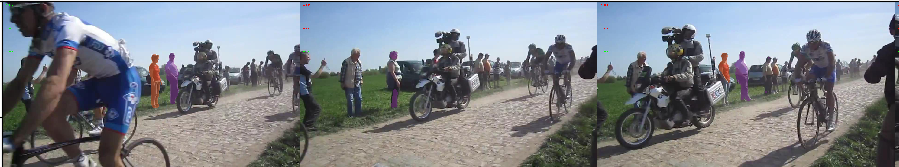
\includegraphics[width=0.9\textwidth]{Figures/aina-occlusion}
\caption{A qualitative example from YouTube-VOS validation of SST handling
         occlusion.}
\label{fig:ainaocclusion}
\end{figure}

We used YouTube-VOS to perform ablation studies on interesting components of
our method, including sparse attention operators and positional encodings.

\begin{table}
\caption{Comparison of positional encoding schemes for the ``grid'' sparse
         attention variant of video attention.}
\centering
\begin{tabular}{lr}
\toprule
Positional Encoding & Grid~\G{} \\
\midrule
None & \num{61.1}  \\
$K$ Embedding & \num{61.8} \\
$T$ Embedding & \num{60.5} \\
$T$ Sinusoidal & \num[math-rm=\mathbf]{62.6} \\
\bottomrule
\end{tabular}
\label{tab:pos-encoding}
\end{table}

In Table~\ref{tab:pos-encoding} we compare the performance of different
positional encoding schemes using the overall score~\G{} on the YouTube-VOS
validation set.
For spatial dimensions we followed \citet{parmar2019standalone} in
using learned relative positional embeddings as the encoding, following Parmar
et al.'s findings that relative are superior to absolute positional embeddings
for spatial attention.
Since we contribute an extension of attention-based models from 2D to 3D, we
focused on experimental investigation of different temporal positional
encodings.

As we described in Equation~\ref{eqn:stridedattndefn}, in sparse video
attention we propagate information through the outer product of query
tensor~$\querytensor_\pixel$ with key tensor~$\keytensor_{I_\pixel}$ indexed by
connectivity pattern~$I_\pixel$.
Adding relative positional embeddings, Equation~\ref{eqn:stridedattndefn} becomes

\begin{equation}
        \mathtt{StridedAttn}{\big(\querytensor, \keytensor, \valuetensor)}_\pixel{} = \softmax\big(\querytensor_\pixel{} \big(\keytensor^\top_{I_\pixel} + \embtensor^\top_{\tilde{I}_\pixel}\big)\big)\keytensor_{I_\pixel}
\end{equation}

\noindent where~$\tilde{I}_\pixel{} = (f(q, \pixel) : q \in I_\pixel)$
is the sequence of relative position indices for points~$q$ in
sequence~$I_\pixel$ relative to pixel~$\pixel$,
and~$f \,:\, \real^3\times \real^3 \rightarrow \real$ is a function mapping
pairs of positions to scalar indices.
For grid attention pixel~$q$ would differ along at most one of the
three spatiotemporal axes~$X, Y, T$, so the relative positional embedding for
pair~$(\pixel, q)$ would correspond to
either~$\Delta_x \equiv q_x - \pixel_x$,
$\Delta_y \equiv q_y - \pixel_y$,~or~$\Delta_t \equiv q_t - \pixel_t$.
For strided attention, the relative positional embedding would be the
concatenation of three separate embeddings corresponding
to~$\Delta_x$,~$\Delta_y$, and~$\Delta_t$.

In addition to relative positional embeddings, we also investigated sinusoidal
positional encodings for the temporal dimension, as used by
\citet{vaswani2017attention} in Transformers for language translation.
We hypothesized that sinusoidal positional encodings would be superior to
absolute positional embeddings because of the data imbalance of absolute
temporal positions in VOS datasets, which are skewed towards lower frame
numbers.
Sinusoidal positional encodings can be interpolated or extrapolated to
generalize to underrepresented absolute frame numbers, whereas absolute
positional embeddings have no such generalization mechanism.
Furthermore, we hypothesized that sinusoidal positional encodings would be
superior to relative positional embeddings because the absolute position
information encoded in the sinusoidal representation encodes information about
a given pixel's temporal distance from the reference frame, whereas relative
positional embeddings encode no information related to distance from the
reference frame.

We present our results comparing different positional encodings in
Table~\ref{tab:pos-encoding} for both grid and strided sparse attention
variants.
The positional encoding labeled ``None'' is our baseline attention with no
positional information, while all remaining positional encodings use relative
positional embeddings for spatial dimensions~$X, Y$.
``$K$ Embedding'' and~``$T$ embedding'' refer to using relative and absolute
temporal positional embeddings, respectively, and~``$T$ sinusoidal'' refers to
using a sinusoidal temporal positional encoding.
Relative temporal positional embeddings outperformed the baseline, while
absolute temporal positional embeddings underperformed the baseline, possibly
due to the data imbalance of absolute temporal positions.
Sinusoidal temporal positional encodings performed best, which is in line with
our hypothesis that information about distance-from-reference is important in
positional encodings for VOS\@.

\begin{table}
\caption{Comparison of sparse and dense evaluation on
         YouTube-VOS~\citep{xu2018youtubevos} for both strided and grid sparse
         attention variants.}
\centering
\begin{tabular}{llr}
\toprule
Method & Evaluation & \G{} \\
\midrule
SST (Grid) & Sparse & \num{65.8} \\
SST (Grid) & Dense & \num{66.5} \\
SST (Strided) & Sparse & \num{66.7} \\
SST (Strided) & Dense & \num[math-rm=\mathbf]{68.1} \\
\bottomrule
\end{tabular}
\label{tab:evalsparse}
\end{table}

At training time we used TSN sampling~\citep{wang2016temporal} to subsample
sequences to a fixed number of frames since backpropagation constrained our
memory usage.
However at test time we do not have the same memory constraint, so we have the
ability to simultaneously predict on an entire sequence of frames at once.
In Table~\ref{tab:evalsparse} we compare the TSN and ``all frames'' test time
sampling methods, which we refer to as sparse and dense evaluation,
respectively.
We show that simultaneously attending to all frames densely produces superior
predictions for both grid and strided sparse attention variants.
We also maintain reasonable accuracy when using TSN sampling at test time to
subsample sequence, showing an advantage of our method over recurrent methods
that would have to process every preceding frame in order to predict on a given
timestep.

% TODO(brendan): grid vs. sparse discussion


\subsection{Discussion}

Our work represents the first algorithm for VOS purely based on end-to-end
attention.
Future work in attention-based models for VOS could be analogous to Transformer
models' progression on language translation tasks, where researchers
successfully applied Transformers to increasingly long sequences.
For example, Dai et al.\ combined recurrence with attention to translate
arbitrary-length sequences~\citep{dai2019transformer}, and Kitaev et al.
introduced locality-sensitive hashing instead of dot-product attention, to
reduce computational complexity from squared to~$O(N\log N)$ while using
reversible networks to model arbitrary-length sequences with constant memory
usage~\citep{kitaev2020reformer}.
In order to evaluate VOS on long sequences the VOS community would have to
overcome a dataset creation challenge, since the current benchmark dataset
YouTube-VOS contains sequences with at most~\num{36} labeled frames, sampled
at~\num{6} frames per second.
We propose that future work could use interactive and semi-automatic annotation
methods, based on the existing high-quality VOS models, to create datasets with
longer and therefore more challenging sequences.


\section{Conclusions}

We presented Sparse Spatiotemporal Transformers (SST), which constitutes the
first application of an entirely attention-based model for video object
segmentation (VOS).
We showed that SST is capable of state-of-the-art results on the benchmark VOS
dataset YouTube-VOS, attaining an overall score of~$\mathcal{G} = \yvosvalG$,
while having superior runtime scalability compared with previous state of the
art methods.
We provide code to reproduce all experiments in our work, including sparse
video-attention operator implementations, so that the community can build on
the promising idea of using attention-based models for video, in the VOS domain
and beyond.

% \chapter{Discussion}

In this thesis we investigated representation learning focused on developing
improved attention and fusion operators for computer vision.
We introduced the idea of learning fusion operators via neural architecture
search, and proposed a search space for fusion operator search for VQA\@.
We demonstrated the potential of our search space by manually finding
configurations of our search space that outperform the baseline fusion model,
MUTAN~\citep{ben2017mutan}, based on Tucker decomposition.
Our improved fusion operator used a gating mechanism to conditionally enable or
disable features, ensembled activation functions, and added additional learned
nonlinearity via a neural network output function.
We showed that our method achieved an absolute percentage point increase
of~\num{1.1}\% in top-1 accuracy over the baseline MUTAN model.
Furthermore, our proposed fusion operator search space holds promise for use
with neural architecture search to discover new, even superior fusion
operators.




% ********************************** Back Matter *******************************
% Backmatter should be commented out, if you are using appendices after References
%\backmatter

% ********************************** Bibliography ******************************
\begin{spacing}{0.9}

% To use the conventional natbib style referencing
% Bibliography style previews: http://nodonn.tipido.net/bibstyle.php
% Reference styles: http://sites.stat.psu.edu/~surajit/present/bib.htm

\bibliographystyle{apalike}
%\bibliographystyle{unsrt} % Use for unsorted references  
%\bibliographystyle{plainnat} % use this to have URLs listed in References
\cleardoublepage
\bibliography{References/references} % Path to your References.bib file


% If you would like to use BibLaTeX for your references, pass `custombib' as
% an option in the document class. The location of 'reference.bib' should be
% specified in the preamble.tex file in the custombib section.
% Comment out the lines related to natbib above and uncomment the following line.

%\printbibliography[heading=bibintoc, title={References}]


\end{spacing}

% ********************************** Appendices ********************************

\begin{appendices} % Using appendices environment for more functunality

%\include{Appendix1/appendix1}
%\include{Appendix2/appendix2}

\end{appendices}

% *************************************** Index ********************************
\printthesisindex % If index is present

\end{document}
